\documentclass[11pt]{article}
\synctex=1

\usepackage{amsmath,amssymb,amsfonts,amsthm,latexsym}
\usepackage{graphicx,booktabs,multirow}
\usepackage{xcolor} % Blue additions for Ivan, November 12, 2026
\usepackage{enumerate,setspace,geometry,changepage,lipsum,xr}
\usepackage[toc,title,titletoc,header]{appendix}
\usepackage{titletoc}
\usepackage{etoc}
\usepackage[bottom]{footmisc}
\usepackage[authoryear]{natbib}
\bibliographystyle{ecta}
\usepackage{xstring} % in preamble

\geometry{letterpaper,left=1in,right=1in,top=1in,bottom=1in}
\setstretch{1.20}
\parskip=1.5ex plus0.5ex minus0.2ex

\numberwithin{equation}{section}

\usepackage[pdfborder={0 0 0},colorlinks=true,linkcolor=magenta,citecolor=blue,filecolor=magenta]{hyperref}
\newcommand{\myref}[2]{\hyperref[#1]{#2}}

\usepackage{lineno,etoolbox}
\setpagewiselinenumbers
% \modulolinenumbers[5]
% \linenumbers

\allowdisplaybreaks

\def\qed{\rule{2mm}{2mm}}
\def\independent{\perp\!\!\!\perp}

\newcommand\undermat[2]{%
  \makebox[0pt][l]{$\smash{\underbrace{\phantom{%
    \begin{matrix}#2\end{matrix}}}_{\text{$#1$}}}$}#2}

\DeclareMathOperator*{\var}{var}
\DeclareMathOperator*{\supp}{supp}

\newtheorem{theorem}{Theorem}
\newtheorem{lemma}{Lemma}
\newtheorem{corollary}{Corollary}
\newtheorem{assumption}{Assumption}
\newtheorem{summary}{Summary}
\newtheorem{definition}{Definition}
\newtheorem{example}{Example}
\newtheorem{remark}{Remark}
\newtheorem{proposition}{Proposition}
\newtheorem{comment}{Comment}
\newtheorem{conjecture}{Conjecture}

\newcounter{assumptionM}
\newcounter{assumptionA}
\def\theassumptionM{M.\arabic{assumptionM}}
\def\theassumptionA{A.\arabic{assumptionA}}
\setcounter{assumptionM}{0}
\setcounter{assumptionA}{0}

\newenvironment{assumptionA}[1][]{%
  \refstepcounter{assumptionA}\medskip\noindent\textbf{Assumption \theassumptionA. #1}%
}{\medskip}

\newenvironment{assumptionM}[1][]{%
  \refstepcounter{assumptionM}\medskip\noindent\textbf{Assumption \theassumptionM. #1}%
}{\medskip}

\AtEndEnvironment{remark}{~\qed}%
\AtEndEnvironment{example}{~\qed}%

% \usepackage{xr,nameref}
% \externaldocument{supp-app}

% -------------------------------------------------------------------------------------------------
\begin{document}
\author{
Federico A. Bugni \\
Department of Economics\\
Northwestern University \\
\url{federico.bugni@northwestern.edu}
\and
Ivan A.\ Canay \\
Department of Economics\\
Northwestern University\\
\url{iacanay@northwestern.edu}
% \and
% Denis Chetverikov \\
% Department of Economics\\
% University of California, Los Angeles\\
% \url{chetverikov@econ.ucla.edu} % TODO: confirm affiliation and email
}

\title{Should We Drop Redundant Moment Inequalities?\footnote{}}
% Alternative title: Testing with Redundant Moment Inequalities

\maketitle

\vspace{-1cm}
\begin{spacing}{1.1}
    \begin{abstract}
    \end{abstract}
\end{spacing}

\noindent KEYWORDS: 

\noindent JEL classification codes: C12, C14.

\thispagestyle{empty}

\newpage 

%%%%%%%%% -------------------------------------------------------------------
\section{Introduction}\label{sec:intro}
%%%%%%%%% -------------------------------------------------------------------
{\color{blue}The introduction is yet to be written. }

{\color{blue}
\noindent\textbf{Papers we should cite:}
\begin{itemize}

\item \citet{galichon/henry:11}: in the introduction when discussing
core-determining classes; in Section~\ref{sec:model} when explaining
that a smaller collection can preserve sharp identification.

\item \citet{chesher/rosen:17}: in the introduction for core-determining
collections in generalized instrumental variable models; in
Section~\ref{sec:model} alongside the identification-sufficiency condition.

\item \citet{chesher/rosen:20}: in the introduction and
Section~\ref{sec:model} to acknowledge that a redundant moment may
be estimated more precisely and help inference
(their Section~9.1, pp.~104--105).

\item \citet{luo/wang:18}: in the introduction for finding smallest
core-determining classes; retain the citation in
Section~\ref{sec:power-two-cores} for their simulation comparison,
without claiming uniform power gains from deletion.

\item \citet*{luo/ponomarev/wang:26}: in the introduction for selecting
inequalities that preserve sharp identification and for their
distinction between identification and inference; retain the citation
in Section~\ref{sec:power-two-cores}.

\item \citet{pakes/porter:24}: {\color{blue}in Section~\ref{sec:model}
for redundancy through nonnegative combinations of inequalities;
optionally in the introduction as a multinomial choice example.}

\item \citet{mbakop:23}: in the introduction for computational
construction and reduction of sharp identifying inequalities; in
Section~\ref{sec:model} for redundancy through nonnegative combinations.

\item \citet*{chernozhukov/chet/kato:19}: in the introduction and
Section~\ref{sec:model} to credit the observation that an inequality
unnecessary for identification can still be useful because of its
precision.

\item \citet{molinari:20}: in the introduction as a synthesis of the
distinction between identification and inference when reducing
inequalities; group with Chesher--Rosen and
Chernozhukov--Chetverikov--Kato rather than repeat the discussion.

\item \citet{ponomarev/semenova:25}: in the introduction, and optionally
Appendix~\ref{app:precision}, as an example of an inferential benefit
from a looser but more precise bound (their Remark~2). Distinguish
their confidence-bound comparison from our comparison of joint tests.

\item \citet{ponomarev:22}: in the introduction when locating our
local-power contribution; retain Section~\ref{sec:power-two-cores}.
Credit comparisons of both the direction and magnitude of power
differences.

\item \citet{manski:04}: optionally in
Section~\ref{sec:power-two-cores} when introducing minimax regret,
as a decision-theoretic precedent in treatment choice, not a source
for our test-specific calculations.

\item \citet{lehmann/romano:05}: retain
Sections~\ref{sec:two-moments} and~\ref{sec:main-lessons} for the
classical admissibility benchmark; mention in the introduction when
explaining what our mean-space restriction changes.

\item \citet{canay/shaikh:2017}: retain Section~\ref{sec:model};
consider their Example~4.1 in Section~\ref{sec:main-lessons} when
connecting our question to the unrestricted Gaussian benchmark.

\end{itemize}
}

%%%%%%%%% -------------------------------------------------------------------
\section{Admissibility in the Normal Model}\label{sec:normal}
%%%%%%%%% -------------------------------------------------------------------

Suppose a collection of moment inequalities suffices to characterize the identified set, so that the remaining inequalities can be discarded without changing it. Should a test use only that collection, or can the remaining inequalities contribute to inference? We study this question first in a normal model, where a subset of the inequalities characterizes the null hypothesis on its own. Our focus here is admissibility: whether a test that retains redundant inequalities can be improved upon uniformly. Section~\ref{sec:population} connects the experiment to the moment inequality model, and Section~\ref{sec:power} measures the power consequences of retaining or discarding redundant inequalities.

\subsection{The Experiment}\label{sec:experiment}

Suppose we observe $X\sim N_d(\mu,\Omega)$, where $\Omega$ is a known positive-definite correlation matrix. Each coordinate has unit variance, so its mean measures a violation in units of its standard deviation. Partition the coordinates $\{1,\dots,d\}$ into two nonempty sets, $\mathcal C$ and $\mathcal R$. We refer to the coordinates in $\mathcal C$ as \emph{core} and to those in $\mathcal R$ as \emph{redundant}, and we maintain that $\mu$ belongs to
\begin{equation}\label{eq:Lambda}
\Lambda:=\Big\{\mu\in\mathbf R^d:\mu_r\le\max_{c\in\mathcal C}\mu_c\ \text{ for every }r\in\mathcal R\Big\}~.
\end{equation}
A positive mean signals a violation of the corresponding inequality. Our interest is in testing the following hypotheses:
\begin{equation}\label{eq:hypotheses}
H_0:\mu\in\Lambda_0:=\Lambda\cap(-\infty,0]^d
\qquad\text{versus}\qquad
H_1:\mu\in\Lambda_1:=\Big\{\mu\in\Lambda:\max_{c\in\mathcal C}\mu_c>0\Big\}~.
\end{equation}
The restriction in \eqref{eq:Lambda} has two implications. First, $\mu\le0$ if and only if $\mu_c\le0$ for every $c\in\mathcal C$, so the core inequalities characterize the null hypothesis on their own. This is the sense in which the remaining inequalities are redundant, corresponding to inequalities that do not affect the identified set in the moment inequality model discussed below. Second, it bounds each redundant mean by the largest core mean, including under the alternative. This ordering is stronger than redundancy alone: it also prevents a redundant coordinate from having a stronger signal than every core coordinate. We impose it to rule out an immediate reason for retaining redundant moments, namely that a moment unnecessary for describing the null may provide the strongest signal against it. Section~\ref{sec:modified-experiment} considers a more permissive experiment that removes this ordering under the alternative while retaining the same null.

The partition into $\mathcal C$ and $\mathcal R$ is part of the maintained model. It is known, and it is the same for every $\mu\in\Lambda$. What varies with $\mu$ is which core coordinate has the largest mean and, as we will see, which tests have the most power. Assigning a different partition to each alternative would define a different testing problem.

To fix ideas, take $d=3$, $\Omega=I_3$, $\mathcal C=\{1,2\}$, and $\mathcal R=\{3\}$, so that $X_1$, $X_2$, and $X_3$ are independent with unit variances and $\mu_3\le\max\{\mu_1,\mu_2\}$. Under this restriction, $\mu_1\le0$ and $\mu_2\le0$ already imply $\mu_3\le0$, so the third inequality adds nothing to the description of the null hypothesis. In this context, our question amounts to: should a test of $H_0$ use $X_3$?

Section~\ref{sec:population} explains how this experiment arises from moment inequalities and discusses the interpretation and scope of the ordering in \eqref{eq:Lambda}.

Fix $0<\alpha<1$. A test is a measurable function $\psi:\mathbf R^d\to[0,1]$, interpreted as the probability of rejecting $H_0$. It has level $\alpha$ if $\sup_{\mu\in\Lambda_0}E_\mu[\psi(X)]\le\alpha$. A level-$\alpha$ test $\psi$ \emph{weakly dominates} a level-$\alpha$ test $\phi$ if $E_\mu[\psi(X)]\ge E_\mu[\phi(X)]$ for every $\mu\in\Lambda_1$, and it \emph{strictly dominates} $\phi$ if, in addition, the inequality is strict for some $\mu\in\Lambda_1$.

\begin{definition}\label{def:admissible}
A level-$\alpha$ test is \emph{$\alpha$-admissible} if no level-$\alpha$ test strictly dominates it.
\end{definition}

The competitors in Definition~\ref{def:admissible} include randomized tests and tests of any shape. Admissibility is a weak requirement, and an admissible test may have poor power at many alternatives. Its value lies in the converse: an inadmissible test can be replaced by a test with the same level that is at least as powerful at every alternative and more powerful at some.

The tests we study reject when $X$ falls outside an acceptance region $A\subseteq\mathbf R^d$, that is, 
$$\phi_A(x):=I\{x\notin A\}~.$$
We call $A$ \emph{nice} if it is closed, convex, and lower (meaning that $x\in A$ and $y\le x$ imply $y\in A$), and if
\begin{equation}\label{eq:exact-size}
P_0\{X\in A\}=1-\alpha~.
\end{equation}
Because $A$ is lower and $\Lambda_0\subseteq(-\infty,0]^d$, the rejection probability of $\phi_A$ over $\Lambda_0$ is largest at $\mu=0$. Condition \eqref{eq:exact-size} therefore makes $\phi_A$ a level-$\alpha$ test with size attained at the origin. The class includes several familiar tests. The max test rejects when $\max_jX_j$ exceeds a critical value and has a rectangular acceptance region. Tests that reject for large values of $a'X$, with $a\ge0$ and $a\ne0$, are also nice, and so are tests based on $\sum_j(X_j)_+^2$ at any level for which a critical value with exact size exists (the statistic equals zero with positive probability, so this rules out only large values of $\alpha$). Each of these tests can use every coordinate or only the core ones.\footnote{Exact size at the origin alone does not ensure admissibility. To see this, take $d=3$, $\Omega=I_3$, $\mathcal C=\{1,2\}$, and $\mathcal R=\{3\}$. Let $Y:=(X_3-X_1,X_3-X_2)'$ and let $V$ be its covariance matrix. Consider the test that rejects when $Y'V^{-1}Y$ falls below the $\alpha$-quantile of the $\chi^2_2$ distribution. When the means are all equal, the statistic has a $\chi^2_2$ distribution and the rejection probability is $\alpha$. Otherwise, it has a noncentral $\chi^2_2$ distribution and the rejection probability is strictly below $\alpha$. The test therefore has size $\alpha$, attained at the origin, but is strictly dominated by the constant test $\psi\equiv\alpha$, which rejects with probability $\alpha$ independently of the data. The power gain is strict, for example, at $\mu=(1,0,0)\in\Lambda_1$. The original test's acceptance region is neither convex nor lower.}

\subsection{The Role of the Number of Core Moments}\label{sec:core-count}
The number of core coordinates determines what we know about the source of a violation. With one core coordinate, every alternative has $\mu_1>0$ and $\mu_r\le\mu_1$ for every redundant coordinate, so a test can exploit this ordering throughout the alternative. With several core coordinates, the redundant means are bounded by the largest core mean, but the coordinate attaining that maximum can vary across alternatives. A proposed improvement must therefore work even when a particular core mean is arbitrarily negative and another core supplies the violation.

We start by asking what an improvement on an exact-size test must look like. Let $\phi$ be a level-$\alpha$ test with $E_0[\phi(X)]=\alpha$, let $\psi$ be a level-$\alpha$ test that weakly dominates it, and set $h:=\psi-\phi$. Level control gives $E_0[h(X)]\le0$, and dominance along the alternatives $te_c$ with $c\in\mathcal C$ gives $E_0[h(X)]\ge0$ as $t\downarrow0$, so $E_0[h(X)]=0$. Now fix $\mu\in\Lambda_1$. Since $\Lambda_1$ is a cone, $t\mu\in\Lambda_1$ for every $t>0$, and the Gaussian likelihood ratio gives
\begin{equation}\label{eq:expansion}
  \begin{split}
  E_{t\mu}[h(X)]
  &=E_0\Big[h(X)\exp\Big\{t\mu'\Omega^{-1}X-\frac{t^2}{2}\,\mu'\Omega^{-1}\mu\Big\}\Big]\\
  &=t\,\mu'\Omega^{-1}q+O(t^2)~,
  \end{split}
  \end{equation}
  where $q:=E_0[Xh(X)]$. The left side must be nonnegative for every $t>0$, so $\mu'\Omega^{-1}q\ge0$ for every $\mu\in\Lambda_1$. In other words, the net shift in rejection probability, summarized by $\Omega^{-1}q$, must not lower power to first order at any alternative. Thus $\Omega^{-1}q$ must belong to the dual cone
\[
\Lambda_1^*:=\{v\in\mathbf R^d:\mu'v\ge0\ \text{ for every }\mu\in\Lambda_1\}~,
\]
and the shape of this cone depends on the \emph{number} of core coordinates, $|\mathcal C|$.

\begin{lemma}[Dual-cone dichotomy]\label{lem:dual}
(a) If $\mathcal C=\{1\}$, then
\[
\Lambda_1^*
=\Big\{v\in\mathbf R^d:\ v_r\le0\ \text{ for } r\in\mathcal R,\ \ v_1+\sum_{r\in\mathcal R}v_r\ge0\Big\}
=\operatorname{cone}\{e_1,\ e_1-e_r:r\in\mathcal R\}~.
\]
(b) If $|\mathcal C|\ge2$, then $\Lambda_1^*=\{0\}$.
\end{lemma}

\begin{lemma}[First-order restriction]\label{lem:first-order}
Let $\phi$ be a level-$\alpha$ test with $E_0[\phi(X)]=\alpha$, and let $\psi$ be a level-$\alpha$ test that weakly dominates $\phi$. Then $h:=\psi-\phi$ satisfies
\[
E_0[h(X)]=0
\qquad\text{and}\qquad
\Omega^{-1}E_0[Xh(X)]\in\Lambda_1^*~.
\]
In particular, if $|\mathcal C|\ge2$, then $E_0[Xh(X)]=0$.
\end{lemma}

Lemma~\ref{lem:first-order} can be understood through the power expansion in \eqref{eq:expansion}. The two tests have the same rejection probability at the origin. As the mean moves from the origin toward an alternative $\mu$, the initial rate of change in their power difference is $\mu'\Omega^{-1}q$. For $\psi$ to weakly dominate $\phi$, this rate must be nonnegative in every direction allowed by the alternative. With two or more core coordinates, Lemma~\ref{lem:dual} shows that this is possible only if $q=0$. Thus any improvement must preserve both the rejection probability at the origin and the first-order response of power to changes in the mean. Any power gain must come from higher-order terms in the expansion. These restrictions apply to arbitrary tests, including randomized tests.

With one core coordinate, a nonzero first-order power gain can be consistent with dominance. For example, take $d=3$ and $\Omega=I_3$. If $\mathcal C=\{1\}$ and $q$ is a positive multiple of $e_1-e_3$, then $\mu'q$ is proportional to $\mu_1-\mu_3$, which is nonnegative at every alternative because the maintained restriction requires $\mu_3\le\mu_1$. If instead $\mathcal C=\{1,2\}$, the same direction gives a negative slope at $\mu=(0,1,1)$, which is now an allowed alternative. There, coordinate 2 supplies the violation and bounds $\mu_3$. A competitor with such a $q$ would therefore lose power near the origin along that alternative. The one-core restriction permits changes that the two-core model rules out. Whether such a change can actually improve a given test depends on its acceptance region, which we examine next.

The likelihood ratio in \eqref{eq:expansion} depends on $x$ through $\mu'\Omega^{-1}x$, so a direction $a$ in the sample space corresponds to the ray of means $t\Omega a$, $t>0$.

\begin{definition}[Finite and feasible normals]\label{def:normals}
For a closed convex set $A$, let $h_A(a):=\sup_{x\in A}a'x$ denote its support function. A vector $a\ne0$ is a \emph{finite normal} of $A$ if $h_A(a)<\infty$, and it is \emph{feasible} if it belongs to
\[
\mathcal F(\Omega,\Lambda):=\{a\in\mathbf R^d:\ a\ge0,\ \Omega a\in\Lambda\}~.
\]
\end{definition}

Finiteness depends on the acceptance region: $a$ is a finite normal if some halfspace $\{x:\ a'x\le c\}$ contains $A$. Feasibility depends on the experiment: for a nonzero $a\ge0$, it means that the ray of means $t\Omega a$ lies in the maintained model. When $A$ is lower, every finite normal satisfies $a\ge0$. Every nonzero $a\ge0$ is a finite normal of a rectangle with finite upper cutoffs on every coordinate, for example, while the finite normals of a halfspace $\{x:\ a'x\le c\}$ are the positive multiples of $a$. A feasible direction generates a ray of alternatives, since every nonzero $a\in\mathcal F(\Omega,\Lambda)$ satisfies $\Omega a\in\Lambda_1$ (Lemma~\ref{lem:feasible-alternative} in Appendix~\ref{app:proofs-normal}). Feasible support, defined next, asks whether the normals that are both finite and feasible are enough to describe $A$.

\begin{definition}[Feasible support]\label{def:feasible-support}
A nice region $A$ is \emph{feasibly supported} if
\[
A=\bigcap_{a\in F_A}\{x\in\mathbf R^d:\ a'x\le h_A(a)\}~,
\qquad
F_A:=\{a\in\mathcal F(\Omega,\Lambda):\ a\ne0,\ h_A(a)<\infty\}~.
\]
\end{definition}

For a full-dimensional polyhedron, feasible support means that every essential facet of $A$ has a feasible normal.

\begin{proposition}[Feasible support suffices]\label{prop:feasible-support}
If a nice region $A$ is feasibly supported, then $\phi_A$ is $\alpha$-admissible.
\end{proposition}

The idea behind Proposition~\ref{prop:feasible-support} is simple. Along the ray of alternatives $t\Omega a$, the likelihood ratio is proportional to $\exp\{t\,a'x\}$. Any rejections a competitor adds lie inside $A$, where $a'x\le h_A(a)$, so if it gives up rejections beyond the face $\{a'x=h_A(a)\}$, those losses eventually outweigh its gains on that ray. Feasible support means that these faces determine $A$, so a competitor cannot give up rejections anywhere outside $A$. Since it has the same rejection probability at the origin, it cannot add rejections inside $A$ either.

Proposition~\ref{prop:feasible-support} gives a sufficient condition for admissibility with two parts: the acceptance region is nice, and it is feasibly supported. The first is mild, and the familiar tests satisfy it. The second is restrictive. It requires every face that determines $A$ to have a normal $a$ whose ray of means $t\Omega a$ lies in the maintained model, and a face that bounds a redundant coordinate on its own never does. Its normal is $e_r$, and the mean $\Omega e_r$ has $(\Omega e_r)_r=1>\max_{c\in\mathcal C}\Omega_{cr}$, so the redundant mean exceeds every core mean, which is exactly what \eqref{eq:Lambda} rules out. Any test that places a separate cutoff on a redundant coordinate, including the max test that uses $X_3$ in the example of Section~\ref{sec:experiment}, therefore falls outside Proposition~\ref{prop:feasible-support}. This does not make such tests inadmissible, since the condition is only sufficient. Whether it can be relaxed depends on the number of core coordinates, which is where Lemma~\ref{lem:first-order} returns.

Despite the above limitations, Proposition~\ref{prop:feasible-support} already covers the rectangular tests that \emph{ignore} the redundant coordinates.

\begin{corollary}[Core-only rectangles]\label{cor:core-only}
For any $\mathcal C$, any $\mathcal R$, and any positive-definite correlation matrix $\Omega$, let $A_{\mathcal C}:=\bigcap_{c\in\mathcal C}\{x:\ x_c\le\kappa_c\}$ with $P_0\{X\in A_{\mathcal C}\}=1-\alpha$. Then $\phi_{A_{\mathcal C}}$ is $\alpha$-admissible.
\end{corollary}

Discarding the redundant coordinates is therefore safe from the standpoint of admissibility, whatever the number of core coordinates. The question remains whether a rectangular test that also uses the redundant coordinates can be improved upon. The answer depends on the number of core coordinates. Before examining the two cases, we relate feasible support to the stronger condition that every finite normal of $A$ be feasible. With one core coordinate the two conditions coincide, and the finite-normal condition gives the exact characterization of admissibility in Section~\ref{sec:two-moments}.

\begin{proposition}\label{prop:relation}
If every finite normal of a nice region $A$ is feasible, then $A$ is feasibly supported. If $|\mathcal C|=1$, the converse also holds.
\end{proposition}

Feasible support asks only that $A$ be described by supporting halfspaces with feasible normals. The stronger condition asks the same of every finite normal, including the normals of halfspaces already implied by that description. For a polyhedron, for example, any nonzero nonnegative combination of facet normals is again a finite normal. With one core coordinate, $\Lambda$ is defined by linear inequalities, so the feasible normals form a closed convex cone, such combinations remain feasible, and the two conditions coincide. With two or more core coordinates, $\Lambda$ is a union of such cones, one for each core coordinate, and combining feasible normals can produce an infeasible one. The symmetric gate in Section~\ref{sec:three-moments} is an example: it is feasibly supported, but the sum of its two gate normals is not feasible.

\subsubsection*{Two or more core coordinates}

When there are two or more core coordinates, a dominator must match the first moments at the origin, and this allows one of the halfspaces that define $A$ to be left completely unrestricted.

\begin{theorem}[Feasible support plus one halfspace]\label{thm:one-extra}
Suppose that $|\mathcal C|\ge2$, and let $A$ be a nice region of the form
\[
A=A_f\cap\{x:\ u'x\le\kappa\}~,
\qquad
A_f=\bigcap_{a\in G}\{x:\ a'x\le\kappa_a\}~,
\]
where $u\ne0$ and $G\subseteq\mathcal F(\Omega,\Lambda)\setminus\{0\}$. Then $\phi_A$ is $\alpha$-admissible.
\end{theorem}

The theorem separates the description of $A$ into two parts. The set $A_f$ collects constraints with feasible normals, while the additional constraint $u'x\le\kappa$ may have an infeasible normal. With two or more core coordinates, this single departure from feasible support preserves admissibility, provided the resulting region is nice. For a rectangle with one redundant coordinate, the core constraints form $A_f$, since their normals $e_c$ are feasible. The cutoff on the redundant coordinate supplies the additional halfspace. The theorem therefore covers the max test that retains the redundant coordinate in this example, whereas Proposition~\ref{prop:feasible-support} could not determine if such a test was admissible.

The first-moment restriction in Lemma~\ref{lem:first-order} is what allows the additional halfspace to have an infeasible normal. Two consequences follow.

\begin{corollary}[Nonnegative halfspaces]\label{cor:halfspace}
Suppose that $|\mathcal C|\ge2$. For every $a\ge0$ with $a\ne0$, the test $I\{a'X>z_{1-\alpha}\sqrt{a'\Omega a}\}$ is $\alpha$-admissible, where $z_{1-\alpha}$ is the $1-\alpha$ quantile of the standard normal distribution.
\end{corollary}

Corollary~\ref{cor:halfspace} includes vectors $a$ that put all of their weight on redundant coordinates. In particular, the test that rejects for large values of $X_r$ alone is admissible, even though its only face has the infeasible normal $e_r$. Feasibility of every face is therefore not necessary for admissibility when there are two or more core coordinates.

\begin{corollary}[Rectangles with one redundant coordinate]\label{cor:rectangles}
Suppose that $|\mathcal C|\ge2$ and $|\mathcal R|=1$, and let $\Omega$ be any positive-definite correlation matrix. Let $A_\kappa:=\bigcap_{j=1}^d\{x:\ x_j\le\kappa_j\}$ with $P_0\{X\in A_\kappa\}=1-\alpha$. Then $\phi_{A_\kappa}$ is $\alpha$-admissible.
\end{corollary}

In particular, the max test that uses every coordinate is admissible whenever there are at least two core coordinates and one redundant coordinate. In the example of Section~\ref{sec:experiment}, a test may therefore use $X_3$ or ignore it: by Corollaries~\ref{cor:core-only} and~\ref{cor:rectangles}, neither the max test that keeps $X_3$ nor the one that drops it can be improved upon uniformly.

The results above leave open regions that need two or more infeasible facets, including rectangles with several redundant coordinates. Section~\ref{sec:modified-experiment} returns to this question and compares the conclusions with those in a more permissive experiment.

\subsubsection*{One core coordinate}

Suppose now that $\mathcal C=\{1\}$ and $\mathcal R=\{2,\dots,d\}$, so that every redundant mean is bounded above by $\mu_1$, and the core coordinate that supplies every violation is known. This is the case in which Lemma~\ref{lem:first-order} leaves room for a nonzero first-order power difference, and here the way a test uses the redundant coordinates matters for admissibility. A test can put positive weight on every redundant coordinate and remain admissible. Under independence, however, a test that uses them through separate rectangular cutoffs can be improved upon, and the improvement keeps the redundant coordinates. But it does change how they enter the rejection rule.

We first add the redundant coordinates to the test based on $X_1$ alone. For any positive-definite correlation matrix, a sufficiently small positive weight on each of them preserves admissibility.

\begin{corollary}[An augmented halfspace]\label{cor:epsilon}
  Suppose that $\mathcal C=\{1\}$, and let $b\in\mathbf R^d$ satisfy $b_1=0$ and $b_r>0$ for every $r\in\mathcal R$. For every positive-definite correlation matrix $\Omega$, there is $\bar\varepsilon>0$ such that, for every $\varepsilon\in(0,\bar\varepsilon]$, the test $I\{a_\varepsilon'X>z_{1-\alpha}\sqrt{a_\varepsilon'\Omega a_\varepsilon}\}$ with $a_\varepsilon:=e_1+\varepsilon b$ is $\alpha$-admissible.
  \end{corollary}

Now consider the rectangular test, which rejects whenever some coordinate exceeds its own cutoff. Under independence, this test can be improved by replacing the separate cutoff on a redundant coordinate $X_r$ with a cutoff on the sum $X_1+X_r$, calibrated to preserve size.

\begin{theorem}[A gate improves on the rectangle]\label{thm:gate}
  Suppose that $\Omega=I_d$, $\mathcal C=\{1\}$, and $\mathcal R=\{2,\dots,d\}$. Let $A_\kappa:=\bigcap_{j=1}^d\{x:\ x_j\le\kappa_j\}$ with $\prod_{j=1}^d\Phi(\kappa_j)=1-\alpha$. Fix $r\in\mathcal R$ and let $b_r$ be the unique solution to
  \begin{equation}\label{eq:gate-calibration}
  P_0\{X_1\le\kappa_1,\ X_1+X_r\le b_r\}=\Phi(\kappa_1)\Phi(\kappa_r)~.
  \end{equation}
  Then the test with acceptance region
  \[
  A_\kappa^{(r)}:=\{x:\ x_1\le\kappa_1,\ x_1+x_r\le b_r\}\cap\bigcap_{j\notin\{1,r\}}\{x:\ x_j\le\kappa_j\}
  \]
  has size $\alpha$ and strictly dominates $\phi_{A_\kappa}$ at every $\mu\in\Lambda_1$.
  \end{theorem}

The gate has the same size as the rectangle and uses the same coordinates. What changes is how it uses the restriction $\mu_r\le\mu_1$: instead of judging $X_r$ on its own, it judges it together with the core coordinate. Together with Corollary~\ref{cor:epsilon}, this shows that keeping a redundant coordinate and giving it a separate rectangular cutoff are distinct decisions. The first is compatible with admissibility, and under independence the second is not. The distinction does not arise in our results for two or more core coordinates, where the rectangle that keeps a single redundant coordinate is itself admissible (Corollary~\ref{cor:rectangles}). With one core coordinate, the question is not only whether redundant coordinates should enter a test, but also how.


The improvement comes from the likelihood ratio. Relative to the rectangle, the gate rejects some points with a large sum $x_1+x_r$ and accepts some points with a large $x_r$, and the two sets have the same probability at the origin. In the coordinates $(x_1,x_r)$, the likelihood ratio is proportional to $\exp\{\mu_1(x_1+x_r)+(\mu_1-\mu_r)(-x_r)\}$, which is increasing in $x_1+x_r$ and in $-x_r$ because $\mu_1>0$ and $\mu_r\le\mu_1$. Holding the other coordinates fixed, every point the gate adds has a larger sum and a smaller $x_r$ than every point it removes. The gate therefore gains more power than it loses at every alternative, strictly so because the sum is strictly larger and $\mu_1>0$.

\subsection{Two Moments}\label{sec:two-moments}

When $d=2$, $\mathcal C=\{1\}$, and $\mathcal R=\{2\}$, we can say exactly which nice tests are admissible. Let
\[
\Omega_\rho:=\begin{pmatrix}1&\rho\\ \rho&1\end{pmatrix}~,
\qquad -1<\rho<1~,
\]
so that $\Lambda=\{\mu\in\mathbf R^2:\ \mu_2\le\mu_1\}$. For $a\ge0$, the condition $\Omega_\rho a\in\Lambda$ reads $(1-\rho)(a_1-a_2)\ge0$, so
\[
\mathcal F(\Omega_\rho,\Lambda)=\{a\in\mathbf R^2:\ 0\le a_2\le a_1\}
\]
for every $\rho$. The feasible directions do not depend on the correlation, although the likelihood ratio does.

\begin{theorem}\label{thm:two-moments}
Let $d=2$, $\mathcal C=\{1\}$, $\mathcal R=\{2\}$, and $\Omega=\Omega_\rho$ with $-1<\rho<1$. For a nice region $A$, the test $\phi_A$ is $\alpha$-admissible if and only if every finite normal $a$ of $A$ satisfies $a_2\le a_1$.
\end{theorem}

Theorem~\ref{thm:two-moments} turns the sufficient condition into an exact one. Propositions~\ref{prop:feasible-support} and~\ref{prop:relation} can only certify admissibility. With two moments, a single infeasible finite normal is enough to conclude that a test can be improved upon. This extends the conclusion of Theorem~\ref{thm:gate}, in two dimensions, from rectangles under independence to every nice region with an infeasible finite normal, under any correlation.

The test that ignores $X_2$ and rejects when $X_1>z_{1-\alpha}$ is admissible: its finite normals are the positive multiples of $e_1$. The max test and the test based on $(X_1)_+^2+(X_2)_+^2$ are inadmissible for every $\rho$, because $e_2$ is a finite normal of both acceptance regions. Yet $X_2$ can enter an admissible test with full weight. The test that rejects for large $X_1+X_2$ is admissible, and so is the gated test with acceptance region $\{x_1\le\kappa_1,\ x_1+x_2\le b\}$. In two dimensions, then, the redundant coordinate can be used, but only in directions that put at least as much weight on the core coordinate.

Sufficiency in Theorem~\ref{thm:two-moments} follows from Propositions~\ref{prop:feasible-support} and~\ref{prop:relation}; see also \citet[Theorem~6.7.1 and Corollary~6.7.1]{lehmann/romano:05}. Necessity is constructive. Given an infeasible finite normal, the proof in Appendix~\ref{app:proof-two-moments} builds a level-$\alpha$ test that strictly dominates $\phi_A$ at every alternative, either by replacing $A$ with a hull generated by feasible normals and recalibrating it to exact size or, when $\rho<0$ and $A$ is not lower along the direction $(1,\rho)$, by a monotone rearrangement of $A$ in $X_1$ with $X_2-\rho X_1$ held fixed. Whether the same characterization holds with one core coordinate and several redundant coordinates is open.

\subsection{Three Moments}\label{sec:three-moments}

We now return to the example in Section~\ref{sec:experiment}, with $d=3$ and $\Omega=I_3$, and hold one test fixed: the rectangle $A_\kappa=\{x:\ x\le\kappa\}$ with $\prod_{j=1}^3\Phi(\kappa_j)=1-\alpha$. With equal cutoffs, this is the max test. We compare two ways of assigning the coordinates.
\begin{enumerate}[(a)]
\item $\mathcal C=\{1,2\}$ and $\mathcal R=\{3\}$. By Corollary~\ref{cor:rectangles}, $\phi_{A_\kappa}$ is $\alpha$-admissible. In fact, any level-$\alpha$ test that weakly dominates it coincides with it almost surely.
\item $\mathcal C=\{1\}$ and $\mathcal R=\{2,3\}$. By Theorem~\ref{thm:gate}, $\phi_{A_\kappa}$ is strictly dominated at every alternative, and a gate on either redundant coordinate does it.
\end{enumerate}
The same rectangular test is therefore admissible with two core coordinates and uniformly improvable with one. In the latter case, knowing that $\mu_1$ bounds both redundant means allows the gate to improve power at every alternative.

This reversal is less mechanical than it may seem. The mean space in (b) is contained in the one in (a), and restricting the model can only make it easier to improve on a given test. The restriction in (b) buys something specific, though. Consider the gate on coordinates 1 and 3,
\[
A_\kappa^{(3)}=\{x:\ x_1\le\kappa_1,\ x_2\le\kappa_2,\ x_1+x_3\le b_3\}~.
\]
This region is lower and has exact size, so $\phi_{A_\kappa^{(3)}}$ is a level-$\alpha$ test in (a) as well. In (a), however, it loses to the rectangle at some alternatives. Take $\mu=(\mu_1,t,t)$ with $t>0$. This mean is an alternative in (a) for every value of $\mu_1$, but not in (b) once $\mu_1<t$. As $\mu_1\to-\infty$, the constraints that involve $x_1$ hold with probability approaching one, so the gated test rejects essentially only when $X_2>\kappa_2$. The rectangle can also reject when $X_3>\kappa_3$. Their powers converge to
\[
1-\Phi(\kappa_2-t)
\qquad\text{and}\qquad
1-\Phi(\kappa_2-t)\Phi(\kappa_3-t)~,
\]
respectively, and the second is strictly larger. The gate relies on coordinate 1 bounding the redundant means. In the two-core model, however, $\mu_2$ can bound $\mu_3$ while $\mu_1$ is arbitrarily negative. Along these alternatives, the gate loses the opportunity to reject on $X_3$. This illustrates why a pairing that improves power throughout the one-core alternative can fail in the larger model.

Pairing the redundant coordinate with both core coordinates does not produce a dominating test either. The symmetric region $\{x_1\le\kappa,\ x_2\le\kappa,\ x_1+x_3\le b,\ x_2+x_3\le b\}$, with $\kappa$ the cutoff of the max test and $b$ chosen for exact size, has the feasible facet normals $e_1$, $e_2$, $e_1+e_3$, and $e_2+e_3$. It is therefore feasibly supported and admissible in (a) by Proposition~\ref{prop:feasible-support}, even though the sum of the two gate normals, $(1,1,2)$, is a finite normal that is not feasible. It does not dominate the max test, however. With $\alpha=0.10$, the cutoffs are $\kappa\approx1.818$ and $b\approx2.646$, and at $\mu=(0.1,-5,0.1)$ the max test rejects with probability $0.0839$, while the symmetric gate rejects with probability $0.0685$.


\subsection{A Modified Experiment}\label{sec:main-lessons}\label{sec:modified-experiment}

The ordering in \eqref{eq:Lambda} provides a demanding benchmark for retaining redundant inequalities. It prevents a redundant mean from exceeding the largest core mean, under both the null and the alternative. Even under this restriction, admissibility does not require us to discard the redundant inequalities. Core-only rectangles are admissible, but so are several tests that retain redundant coordinates. With one core coordinate, how those coordinates enter the test matters: under independence, a gate improves uniformly on a rectangle while continuing to use them.

With two or more core coordinates, two questions remain open. Is every nice test admissible? More specifically, are rectangles with several redundant coordinates admissible? These questions are natural in light of the unrestricted normal experiment. If the mean space is $\mathbf R^d$, with null $\mu\le0$ and alternative its complement, every nice test is admissible. Every finite normal $a$ of a nice region is nonnegative, and positive definiteness implies that $\Omega a$ has a positive component whenever $a\ne0$. Each normal therefore generates a ray of alternatives, and the classical admissibility criterion applies \citep[Theorem~6.7.1 and Corollary~6.7.1]{lehmann/romano:05}. The ordering in \eqref{eq:Lambda} excludes some of these rays, so the same argument does not settle either question.


We now consider a more permissive experiment. We keep the null $\Lambda_0$, the partition into $\mathcal C$ and $\mathcal R$, and the correlation matrix $\Omega$, but remove the ordering under the alternative. The hypotheses become
\begin{equation}\label{eq:modified-hypotheses}
H_0:\mu\in\Lambda_0
\qquad\text{versus}\qquad
H_1:\mu\in\widetilde\Lambda_1
:=\Big\{\mu\in\mathbf R^d:\max_{c\in\mathcal C}\mu_c>0\Big\}~,
\end{equation}
with maintained mean space $\widetilde\Lambda:=\Lambda_0\cup\widetilde\Lambda_1$. The core inequalities still characterize the null, but redundant means can now exceed every core mean by an arbitrary amount under the alternative.

In this experiment, a condition on the correlation matrix suffices for every nice test to be admissible. The condition asks whether some nonnegative weighted average of the core components has nonnegative covariance with every component of $X$. Formally, there exists $w\in\mathbf R^{|\mathcal C|}$ such that
\begin{equation}\label{eq:core-average}
  w_c\ge0\quad(c\in\mathcal C)~,
  \qquad
  \sum_{c\in\mathcal C}w_c=1~,
  \qquad
  \sum_{c\in\mathcal C}\Omega_{jc}w_c\ge0
  \quad\text{for every }j=1,\dots,d~.
\end{equation}
The weights describe a property of $\Omega$; they need not be used by the test. Independence satisfies this condition, as does any correlation matrix with nonnegative correlations between core and redundant coordinates. The condition also allows some of these correlations to be negative.


\begin{theorem}[Admissibility in the modified experiment]\label{thm:modified-nice}
Suppose that \eqref{eq:core-average} holds. In the experiment \eqref{eq:modified-hypotheses}, $\phi_A$ is $\alpha$-admissible for every nice region $A$, for any number of core and redundant coordinates.
\end{theorem}

The added alternatives allow the supporting-halfspace argument to apply to every face of a nice region. Under \eqref{eq:core-average}, each nonnegative normal $a\ne0$ has a core component of $\Omega a$ that is nonnegative. Its ray of means therefore lies in the enlarged alternative or can be approached by alternatives. This is enough to rule out a uniform improvement, by the same argument that underlies Proposition~\ref{prop:feasible-support}. The proof is in Appendix~\ref{app:modified-experiment}.


Theorem~\ref{thm:modified-nice} changes the answer for the one-core rectangle under independence. In the original experiment, Theorem~\ref{thm:gate} supplies a gate that strictly improves on it at every alternative. In the modified experiment, the rectangle is admissible. The gate remains level $\alpha$, since the null has not changed, but it loses to the rectangle at some of the added alternatives. The ordering provides information about the alternative that makes a uniform improvement possible. Removing that information requires the test to perform well over a larger set of alternatives.

For rectangles, the correlation condition can be weakened. It is enough that each redundant component have nonnegative correlation with at least one core component; the core component need not be the same for all redundant components. Under this condition, every rectangle with finite cutoffs and exact size is admissible in the modified experiment. With two or more cores, the conclusion holds even if one redundant component is negatively correlated with every core component. Appendix~\ref{app:modified-experiment} establishes these results.

Some restriction on correlation is nevertheless needed to conclude that every nice test is admissible. With one core, if a redundant component is negatively correlated with the core component, the test that rejects for large values of that redundant component alone can be improved upon uniformly. The appendix gives the improving test.

Admissibility does not tell us how much power is at stake when we keep or drop redundant inequalities. Consider again the original experiment with two core components and one redundant component. The max test using only the core components and the max test using all three components are both admissible, and each is more powerful than the other at some alternatives.\footnote{The proofs of Proposition~\ref{prop:feasible-support} and Theorem~\ref{thm:one-extra} show that any weak dominator of either test coincides with it almost surely. Since the two tests differ, neither can weakly dominate the other.} The remaining question is how large these gains and losses can be. Section~\ref{sec:power} quantifies them.

Admissibility does not measure the power consequences of retaining or discarding redundant inequalities. Returning to the original experiment, the two max tests in case (a) of Section~\ref{sec:three-moments} are both admissible. The proofs of Proposition~\ref{prop:feasible-support} and Theorem~\ref{thm:one-extra} show that any weak dominator of either test coincides with it almost surely. Since the tests differ, each is more powerful at some alternatives. Section~\ref{sec:power} measures how much.



%%%%%%%%% -------------------------------------------------------------------
\section{From Population Inequalities to the Normal Experiment}\label{sec:population}
%%%%%%%%% -------------------------------------------------------------------

We now consider a moment inequality model in which a collection of inequalities has been shown to characterize the identified set. The question is whether a test should use only that collection. We first distinguish what the identification argument establishes from the additional ordering imposed in Section~\ref{sec:experiment}. This distinction matters because inference compares violations relative to their sampling variability. We then connect the tests to the original ordered experiment. Identification redundancy alone implies neither its ordering nor the unrestricted alternative in Section~\ref{sec:modified-experiment}.

\subsection{The Moment Inequality Model}\label{sec:model}

Let $W_i$, $i=1,\dots,n$, be an i.i.d.\ sequence of random vectors with distribution $P\in\mathbf P$ on $\mathbf R^{d_W}$, and let $m=(m_1,\dots,m_d)'$ be a known measurable function of $W_i$ and a parameter $\theta\in\Theta$. Write $\mu(\theta,P):=E_P[m(W_i,\theta)]$. The identified set is
\begin{equation}\label{eq:identified-set}
\Theta_0(P):=\{\theta\in\Theta:\ \mu(\theta,P)\le0\}~.
\end{equation}
Suppose an identification argument provides a partition of $\{1,\dots,d\}$ into nonempty sets $\mathcal C$ and $\mathcal R$ such that
\begin{equation}\label{eq:id-redundancy}
\Theta_0(P)=\{\theta\in\Theta:\ \mu_c(\theta,P)\le0\text{ for every }c\in\mathcal C\}
\qquad\text{for every }P\in\mathbf P~.
\end{equation}
The inequalities in $\mathcal C$ suffice to characterize the identified set, and those in $\mathcal R$ are \emph{redundant for identification}. We refer to $\mathcal C$ as the core collection. It could be a smallest such collection, but \eqref{eq:id-redundancy} requires only sufficiency. We take the partition as given and keep it fixed over the maintained model. Our question is whether the recommendation to use only $\mathcal C$ also makes sense for inference.

Redundancy can arise in several ways. For example, if $\mu_3(\theta,P)=\mu_1(\theta,P)+\mu_2(\theta,P)$, the first two inequalities imply the third, even though the third mean exceeds both core means when they are positive. The sum here is a relation between means; it does not require the random moments themselves to add up or their covariance matrix to be singular. More generally, an inequality may follow from a nonnegative combination of the core inequalities.

For identification, the signs of the means are enough to determine whether a parameter value belongs to the identified set. For inference, the size of a violation relative to its sampling variability also matters. Let $\sigma_j^2(\theta,P)>0$ denote the variance of $m_j(W_i,\theta)$, let $D(\theta,P)$ be the diagonal matrix of these standard deviations, and let $\Omega(\theta,P)$ denote the correlation matrix of $m(W_i,\theta)$. Dividing each mean by its standard deviation preserves its sign. Thus the same collection $\mathcal C$ characterizes the identified set before and after this normalization; if it is a smallest such collection, it remains one. What can change is the ranking of the violations. A redundant moment can have the largest violation relative to its standard deviation, as Example~\ref{ex:redundancy-precision} illustrates.

\begin{example}[Identification redundancy and precision]
  \label{ex:redundancy-precision}
  Suppose that $\theta\in\mathbf R$ and
  \[
  \mu_1(\theta,P)=\theta-1~,
  \qquad
  \mu_2(\theta,P)=\theta-2~,
  \]
  with standard deviations $\sigma_1(\theta,P)=2$ and $\sigma_2(\theta,P)=1/2$. The identified set is $\Theta_0(P)=(-\infty,1]$, and the second inequality is redundant: every parameter value it excludes is already excluded by the first. Studentization leaves these restrictions unchanged, since
  \[
  \frac{\theta-1}{2}\le0 \iff \theta\le1~,
  \qquad
  2(\theta-2)\le0 \iff \theta\le2~.
  \]
  Nevertheless, at $\theta=3$ the standardized violations are $1$ and $2$, respectively. The redundant inequality therefore has the larger violation relative to its sampling variability, even though its mean is smaller. The second inequality remains redundant for identification, but it provides the stronger standardized signal at this alternative. Our ordering rules out this possibility. This makes admissibility harder to establish, since a competing test has fewer alternatives over which it must do at least as well. We ask whether retaining redundant moments can be justified even under this restriction.
\end{example}

Following \citet{canay/shaikh:2017}, we construct confidence sets for points in $\Theta_0(P)$ by inverting tests of
\[
H_\theta:\ \mu(\theta,P)\le0~.
\]
A test $\phi_n(\theta)$ of $H_\theta$ is uniformly consistent in level if
\begin{equation}\label{eq:uniform-level}
\limsup_{n\to\infty}\ \sup_{P\in\mathbf P}\ \sup_{\theta\in\Theta_0(P)}E_P[\phi_n(\theta)]\le\alpha~.
\end{equation}
The hypothesis does not depend on the units in which the moments are measured. Replacing $m_j$ by $c_jm_j$, for positive constants $c_j$ that may depend on $\theta$, leaves every sign unchanged. It is natural to require the same invariance of a test: changing units should not change the conclusion drawn from the data. The familiar procedures achieve this by using studentized moments. Let $\bar m_n(\theta)$, $\hat D_n(\theta)$, and $\hat\Omega_n(\theta)$ denote the sample mean, diagonal matrix of sample standard deviations, and sample correlation matrix. The tests reject for large values of
\begin{equation}\label{eq:Tn}
T_n(\theta):=T\big(\hat D_n^{-1}(\theta)\sqrt n\,\bar m_n(\theta),\ \hat\Omega_n(\theta)\big)~,
\end{equation}
where $T$ is continuous and weakly increasing in each component of its first argument. Examples include the max statistic $\max_jx_j$, the modified method of moments statistic $\sum_j(x_j)_+^2$, and the quasi-likelihood ratio statistic $\inf_{t\le0}(x-t)'\Omega^{-1}(x-t)$; see \citet{canay/shaikh:2017} and \citet{canay/illanes/velez:26}. The test is $\phi_n(\theta):=I\{T_n(\theta)>\hat c_n(1-\alpha,\theta)\}$, with a critical value chosen so that \eqref{eq:uniform-level} holds. Rescaling a moment multiplies its sample mean and standard deviation by the same factor and leaves the sample correlations unchanged. It therefore leaves \eqref{eq:Tn} unchanged, as well as the critical values considered below. The same construction can be applied to the core moments alone; both retaining and discarding the redundant moments are compatible with scale-invariant inference.

Identification redundancy therefore leaves open whether a redundant moment has the strongest standardized violation. To express the ordering studied in Section~\ref{sec:normal} in the population model, we impose the additional restriction
\begin{equation}\label{eq:standardized-order}
\frac{\mu_r(\theta,P)}{\sigma_r(\theta,P)}\le\max_{c\in\mathcal C}\frac{\mu_c(\theta,P)}{\sigma_c(\theta,P)}
\qquad\text{for every }r\in\mathcal R,\ \theta\in\Theta,\text{ and }P\in\mathbf P~.
\end{equation}
This uses the same fixed partition as \eqref{eq:id-redundancy}, but asks for more: no redundant moment has a larger standardized mean than every core moment. It does not directly follow from identification redundancy. It is a maintained restriction on the signals, expressed on the scale used for inference. It is unchanged by positive rescaling of the moment functions.

The next subsection shows how \eqref{eq:standardized-order} leads to the ordered mean space $\Lambda$ in \eqref{eq:Lambda}.

\subsection{Local Alternatives}\label{sec:local}

Consider sequences $\{(\theta_n,P_n)\}_{n\ge1}$ with $\theta_n\in\Theta$ and $P_n\in\mathbf P$ such that
\begin{equation}\label{eq:local}
D(\theta_n,P_n)\to D~,
\qquad
\Omega(\theta_n,P_n)\to\Omega~,
\qquad
\sqrt n\,D^{-1}(\theta_n,P_n)\,\mu(\theta_n,P_n)\to \delta\in\mathbf R^d~,
\end{equation}
where $D=\operatorname{diag}(\sigma_1,\dots,\sigma_d)$ has positive diagonal entries and $\Omega$ is positive definite. The vector $\delta$ measures the local violation of each inequality in units of its standard deviation. Under the uniform integrability condition of \citet{andrews/soares:10} and \citet{romano/shaikh/wolf:14}, the studentized moments have a Gaussian limit along these sequences. Under $P_n$,
\begin{equation}\label{eq:gaussian-limit}
X_n:=\hat D_n^{-1}(\theta_n)\sqrt n\,\bar m_n(\theta_n)\ \stackrel{d}{\to}\ X\sim N_d(\delta,\Omega)
\qquad\text{and}\qquad
\hat\Omega_n(\theta_n)\ \stackrel{P}{\to}\ \Omega~.
\end{equation}
Proposition~\ref{prop:local-limit} in Appendix~\ref{app:local-limits} states this result formally. Null sequences have $\delta\le0$, while $\max_{c\in\mathcal C}\delta_c>0$ implies that $\theta_n$ lies outside the identified set for all sufficiently large $n$. Under the standardized order in \eqref{eq:standardized-order}, the limiting mean satisfies $\delta\in\Lambda$. Thus $\delta$ plays the role of $\mu$ in Section~\ref{sec:normal}, and the limit has the same correlation matrix $\Omega$.

The underlying moment model may impose additional restrictions on the attainable local means and their covariance matrix. In particular, a test that is admissible in our Gaussian experiment may be improvable on the smaller family of distributions allowed by additional restrictions from the economic model. We abstract away from such additional restrictions and take the ordered Gaussian experiment in Section~\ref{sec:experiment} as the relevant limit experiment.

To see why redundant inequalities remain relevant in the limit, consider the tests in \eqref{eq:Tn} using generalized moment selection with a diverging threshold \citep{andrews/soares:10,Bugni:10,canay:10a}. Let $\kappa_n\to\infty$ with $\kappa_n/\sqrt n\to0$, and let $\hat s_n(\theta)$ have $j$th component equal to $0$ if $\sqrt n\,\bar m_{n,j}(\theta)/\hat\sigma_{n,j}(\theta)>-\kappa_n$ and to $-\infty$ otherwise. The critical value $\hat c_n(1-\alpha,\theta)$ is the $1-\alpha$ quantile of $T(Z+\hat s_n(\theta),\hat\Omega_n(\theta))$, where $Z\sim N_d(0,\hat\Omega_n(\theta))$, or a bootstrap approximation to it, under conditions that make the bootstrap consistent. Along \eqref{eq:local}, $X_n/\kappa_n\to0$ in probability, so every inequality is selected with probability approaching one. If the distribution of $T(Z,\Omega)$ with $Z\sim N_d(0,\Omega)$ is continuous and strictly increasing at its $1-\alpha$ quantile $c_{1-\alpha}$, the critical value converges in probability to $c_{1-\alpha}$, and the limiting rejection probability is $P\{T(Z+\delta,\Omega)>c_{1-\alpha}\}$. This is the power of the test $\phi_A$ of Section~\ref{sec:normal} with acceptance region
\[
A=\{x\in\mathbf R^d:\ T(x,\Omega)\le c_{1-\alpha}\}~.
\]
The region is closed and lower, it has exact size, and it is convex for the three statistics above. The limits of these tests are therefore \emph{nice} tests in the sense of Section~\ref{sec:normal}. Procedures with non-drifting tuning parameters, such as the two-step test of \citet{romano/shaikh/wolf:14} with a fixed first-step level, can retain data-dependent critical values in the limit and require a separate analysis.

Moment selection removes an inequality only outside the finite-drift regime of \eqref{eq:local}. Let $\delta_{n,j}$ denote the $j$th component of $\sqrt n\,D^{-1}(\theta_n,P_n)\mu(\theta_n,P_n)$. If $\delta_{n,j}/\kappa_n\to-c$ with $1<c\le\infty$, as when $\mu_j(\theta_n,P_n)$ stays below a fixed negative number, the $j$th inequality is dropped with probability approaching one, and, if the remaining coordinates satisfy the conditions in \eqref{eq:local}, the limit is the normal model in those coordinates. This distinguishes deletion based on slackness from deletion based on identification redundancy. The former uses the distance from the boundary; the latter uses an implication among population inequalities. A redundant inequality with a finite local drift is retained, so moment selection does not settle the question we study. Moment selection also cannot tell which core inequality supplies the violation. Within the normal model, two means whose largest core coordinates differ give mutually absolutely continuous distributions, so no rule based on $X$ identifies the larger core mean with probability one under both. The uncertainty about the source of a violation that drives the results for two or more core coordinates in Section~\ref{sec:core-count} is therefore present in the Gaussian limit.

%%%%%%%%% -------------------------------------------------------------------
\section{Local Power}\label{sec:power}
%%%%%%%%% -------------------------------------------------------------------

% Status (Nov 10): first draft by Luke from R2-D2's Section 4 plan (R2-Luke-outputs/section4-plan.tex).
% Figures 1-3 are R2-D2's deterministic prototypes, copied unchanged into figures/ as sec4-pilot-*.pdf;
% they are provisional and should be replaced by production versions.

We return to the original ordered experiment, using the three-inequality model of Section~\ref{sec:three-moments} to measure the power at stake when we keep or drop redundant inequalities. With two core inequalities, the max tests that keep and drop the redundant inequality are both admissible, and we measure the losses from either choice. We then impose the one-core restriction, under which a gate improves on the same three-coordinate max test. The calculations show how much this improvement is worth, how the gate compares with dropping the redundant inequalities, and why its dominance fails when we return to two cores.

Let $X\sim N_3(\delta,I_3)$, where $\delta$ is the vector of standardized local violations in \eqref{eq:local}, and set $\alpha=0.10$. For a set of coordinates $J\subseteq\{1,2,3\}$, the max test on $J$ rejects when $\max_{j\in J}X_j>c_{|J|}$, where $c_k:=\Phi^{-1}\big((1-\alpha)^{1/k}\big)$ is the critical value of the max statistic on $k$ independent coordinates. Its power is
\begin{equation}\label{eq:max-power}
\beta_J(\delta):=1-\prod_{j\in J}\Phi\big(c_{|J|}-\delta_j\big)~,
\end{equation}
and $(c_1,c_2,c_3)\approx(1.28,\,1.63,\,1.82)$. Each of these tests rejects with probability $\alpha$ at $\delta=0$ and has level $\alpha$, because $\delta\le0$ under the null hypothesis. A test that uses more coordinates has more opportunities to reject, but it needs a larger critical value, and this is the trade-off whenever we compare max tests on different sets of coordinates. We report differences in power in percentage points. All numbers come from \eqref{eq:max-power} or from a one-dimensional integral, and none involves simulation. We do not weight the alternatives, so the figures show where a test gains or loses and by how much, not how often.

\subsection{Two Cores and One Redundant Inequality}\label{sec:power-two-cores}

First take $\mathcal C=\{1,2\}$ and $\mathcal R=\{3\}$. The maintained order is $\delta_3\le\max\{\delta_1,\delta_2\}$, and the alternatives satisfy $\max\{\delta_1,\delta_2\}>0$. The max test on $\{1,2\}$ and the max test on $\{1,2,3\}$ are both admissible, by Corollaries~\ref{cor:core-only} and~\ref{cor:rectangles}, so each is more powerful than the other at some alternatives. By \eqref{eq:max-power}, the gain in power from keeping the redundant inequality is
\begin{equation}\label{eq:keep-minus-drop}
\Delta(\delta):=\beta_{\{1,2,3\}}(\delta)-\beta_{\{1,2\}}(\delta)=A_2-A_3\,\Phi(c_3-\delta_3)~,
\qquad
A_k:=\Phi(c_k-\delta_1)\Phi(c_k-\delta_2)~,
\end{equation}
which is strictly increasing in $\delta_3$. We therefore fix the core signals $(\delta_1,\delta_2)$ and let the redundant signal vary over its allowed range. Keeping the redundant inequality costs the most when $\delta_3$ is very negative, because $X_3$ then almost never exceeds its cutoff and yet the cutoff is $c_3$ instead of $c_2$. Dropping it costs the most when $\delta_3$ is as large as the order allows. The two costs are
\begin{equation}\label{eq:K-L}
K(\delta_1,\delta_2):=A_3-A_2
\qquad\text{and}\qquad
L(\delta_1,\delta_2):=\big[A_2-A_3\,\Phi\big(c_3-\max\{\delta_1,\delta_2\}\big)\big]_+~,
\end{equation}
where $[x]_+:=\max\{x,0\}$. The first is the largest loss from keeping, approached as $\delta_3\to-\infty$, and the second is the largest loss from dropping, attained at $\delta_3=\max\{\delta_1,\delta_2\}$ when it is positive. For every allowed $\delta_3$, $-K\le\Delta(\delta)\le L$. The two bounds refer to different alternatives, and no alternative incurs both.

To fix ideas, let $\delta_1=\delta_2=1$. The test that drops the redundant inequality has power $45.8\%$. The test that keeps it has power $37.1\%$ when $\delta_3=-4$, $39.2\%$ when $\delta_3=0$, and $50.1\%$ when $\delta_3=1$, and the two powers are equal at $\delta_3\approx0.73$. At $\delta_3=0.9$, keeping gains $2.6$ points although the redundant violation is smaller than both core violations, so a redundant inequality need not carry the largest signal to be useful. When the second core inequality is slack, as in $\delta=(1,-2,1)'$, the power is $26.4\%$ without the redundant inequality and $37.1\%$ with it.

\begin{figure}[t]
\centering
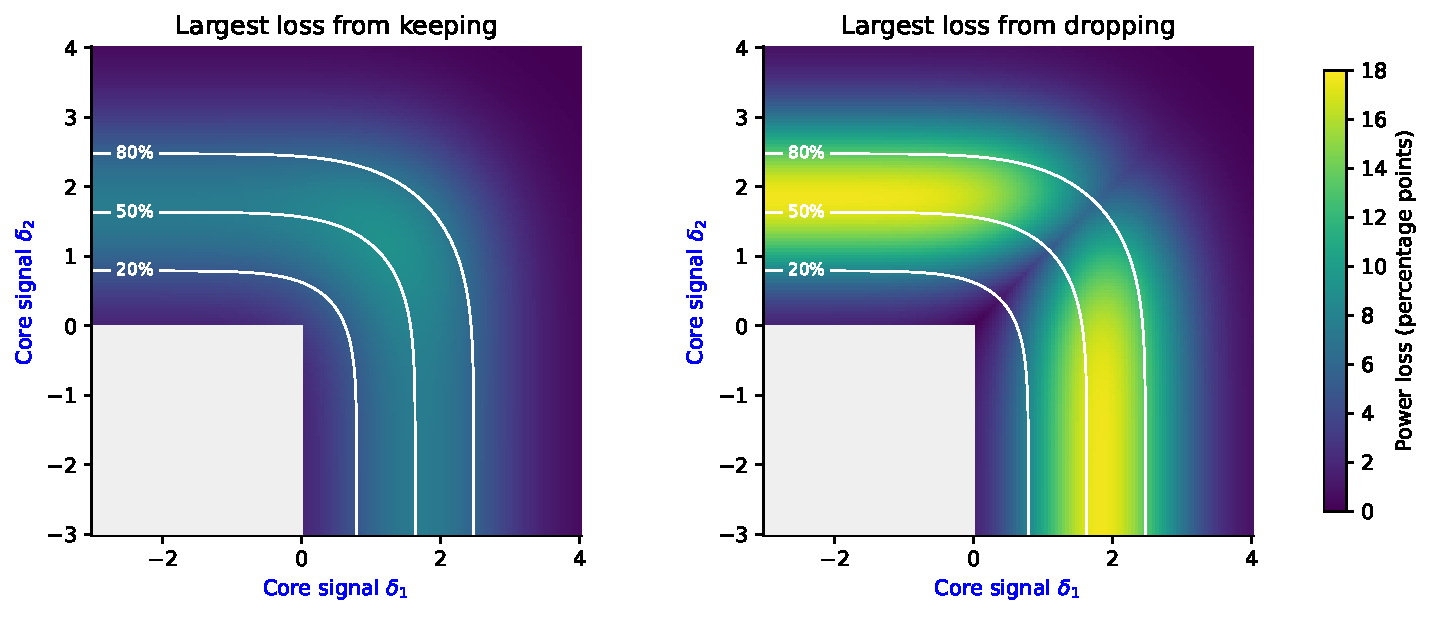
\includegraphics[width=\textwidth]{figures/sec4-pilot-envelopes.pdf}
\caption{Largest loss in power from keeping the redundant inequality, $K$ (left), and from dropping it, $L$ (right), defined in \eqref{eq:K-L}, as functions of the core signals. Two core inequalities, independent moments with a common scale, $\alpha=0.10$. The white curves are the points at which the max test on $\{1,2\}$ has power $20\%$, $50\%$, and $80\%$. The gray region is the null hypothesis.}
\label{fig:envelopes}
\end{figure}

Figure~\ref{fig:envelopes} shows $K$ and $L$ over a range of core signals. The largest losses arise at intermediate core signals, and both costs vanish as the largest core signal grows. In this design, the cost of keeping has a maximum of about $9.04$ points, at $\delta_1=\delta_2\approx1.22$. The cost of dropping is larger. Its supremum is about $17.63$ points, approached when one core signal is near $1.85$ and the other core inequality is far from binding. At such alternatives, the redundant inequality can match the only core inequality that is violated, and the test that keeps it has two informative coordinates where the test that drops it has one. Along the diagonal $\delta_1=\delta_2$, where the redundant inequality would be a third informative coordinate instead of a second, the cost of dropping peaks at about $6.2$ points.

These comparisons also have a minimax-regret interpretation. At each alternative, define the regret of a test as its loss in power relative to the better of the two tests. The regrets from keeping and dropping are therefore $[-\Delta(\delta)]_+$ and $[\Delta(\delta)]_+$, respectively. At fixed core signals, $K$ and $L$ give their largest values over the redundant signal. Taking the supremum over all alternatives gives maximum regrets of about $9.04$ percentage points from keeping and $17.63$ from dropping. For this design, minimax regret favors retaining the redundant inequality among these two tests. Both tests are admissible, but keeping has the smaller worst-case loss, even though our restriction prevents the redundant inequality from having a larger signal than both core inequalities.

The cost of keeping requires one qualification. The quantity $K$ is a supremum over finite values of $\delta_3$, for which the critical value remains $c_3$. This is a different limit from one in which the third inequality is slack enough for moment selection to remove it. If $\delta_{n,3}/\kappa_n\to-c$ with $c>1$ while the core drifts remain finite, as in Section~\ref{sec:local}, the third inequality is dropped with probability approaching one, the limiting critical value is $c_2$, and the loss disappears. Thus $K$ measures the cost of a redundant inequality that is slack, but not slack enough for moment selection to remove it.

Comparisons of this kind have precedents. \citet[Section~2.3.3]{ponomarev:22} compares the local power of studentized max tests that use two core inequalities with and without a third inequality that they imply, and reports gains from including it in his designs when both core inequalities are violated. There, the third statistic is a linear combination of the first two, so it adds a direction in which to reject but no sampling variation of its own, and, in the original units, the third violation is the sum of the core violations instead of being bounded by the larger of them. \citet[Section~5.3]{luo/wang:18} report simulations for an entry game in which removing the redundant inequalities raises rejection rates along one sequence of alternatives. \citet[Section~4.3.1]{luo/ponomarev/wang:26} also distinguish redundancy for identification from usefulness for inference, noting that the power comparison depends on the alternatives of interest. In our comparison the redundant moment has its own sampling variation, and we bound both the gain and the loss at given core signals.

\subsection{One Core}\label{sec:power-one-core}

Now impose $\delta_2,\delta_3\le\delta_1$, so that $\mathcal C=\{1\}$ and $\mathcal R=\{2,3\}$. At every alternative, $\delta_1>0$, and we know which core mean bounds the redundant ones. Theorem~\ref{thm:gate} uses this knowledge to improve uniformly on the three-coordinate max test that was admissible in Section~\ref{sec:power-two-cores}. We compare the size of this improvement with the gains and losses from dropping the redundant inequalities. There are three tests. The first uses only the core inequality and rejects when $X_1>c_1$; it is admissible by Corollary~\ref{cor:core-only}. The second is the max test on $\{1,2,3\}$, the rectangle of Section~\ref{sec:three-moments}. The third is the gate of Theorem~\ref{thm:gate} on coordinates 1 and 3, with acceptance region
\[
\{x\in\mathbf R^3:\ x_1\le c_3,\ x_2\le c_3,\ x_1+x_3\le b\}~,
\]
where $b\approx2.34$ solves \eqref{eq:gate-calibration} with $\kappa_1=\kappa_3=c_3$. The pairing is chosen before seeing the data, and the other redundant coordinate keeps its rectangular cutoff. The power of the gate is
\begin{equation}\label{eq:gate-power}
\beta_G(\delta):=1-\Phi(c_3-\delta_2)\int_{-\infty}^{c_3}\varphi(x-\delta_1)\,\Phi(b-x-\delta_3)\,dx~,
\end{equation}
where $\varphi$ is the standard normal density. Theorem~\ref{thm:gate} gives $\beta_G(\delta)>\beta_{\{1,2,3\}}(\delta)$ at every alternative. It leaves open how much power is gained and how the gate compares with the core-only test; it also does not establish admissibility of the gate.

It is convenient to write the alternatives as $\delta=(s,\ s-g_2,\ s-g_3)'$ with $s>0$ and $g_2,g_3\ge0$, where $s$ is the core signal and $g_r$ measures how slack redundant inequality $r$ is relative to the core inequality. We set $s=c_1$, so that the core-only test has power $50\%$ whatever the values of $g_2$ and $g_3$. Table~\ref{tab:one-core} reports the power of the three tests at four alternatives, and Figure~\ref{fig:gate} shows the three pairwise differences for $g_2,g_3\in[0,6]$.

\begin{table}[!ht]
\centering
\begin{tabular}{ccccc}
\toprule
$g_2$ & $g_3$ & Core-only & Rectangle & Gate on $(1,3)$\\
\midrule
0 & 0 & 50.00 & 65.07 & 71.34\\
3 & 0 & 50.00 & 50.41 & 59.31\\
0 & 3 & 50.00 & 50.41 & 50.51\\
3 & 3 & 50.00 & 29.60 & 29.75\\
\bottomrule
\end{tabular}
\caption{Power, in percent, with one core inequality at $\delta=(s,\ s-g_2,\ s-g_3)'$ and $s=c_1$. Independent moments with a common scale, $\alpha=0.10$.}
\label{tab:one-core}
\end{table}

\begin{figure}[t]
\centering
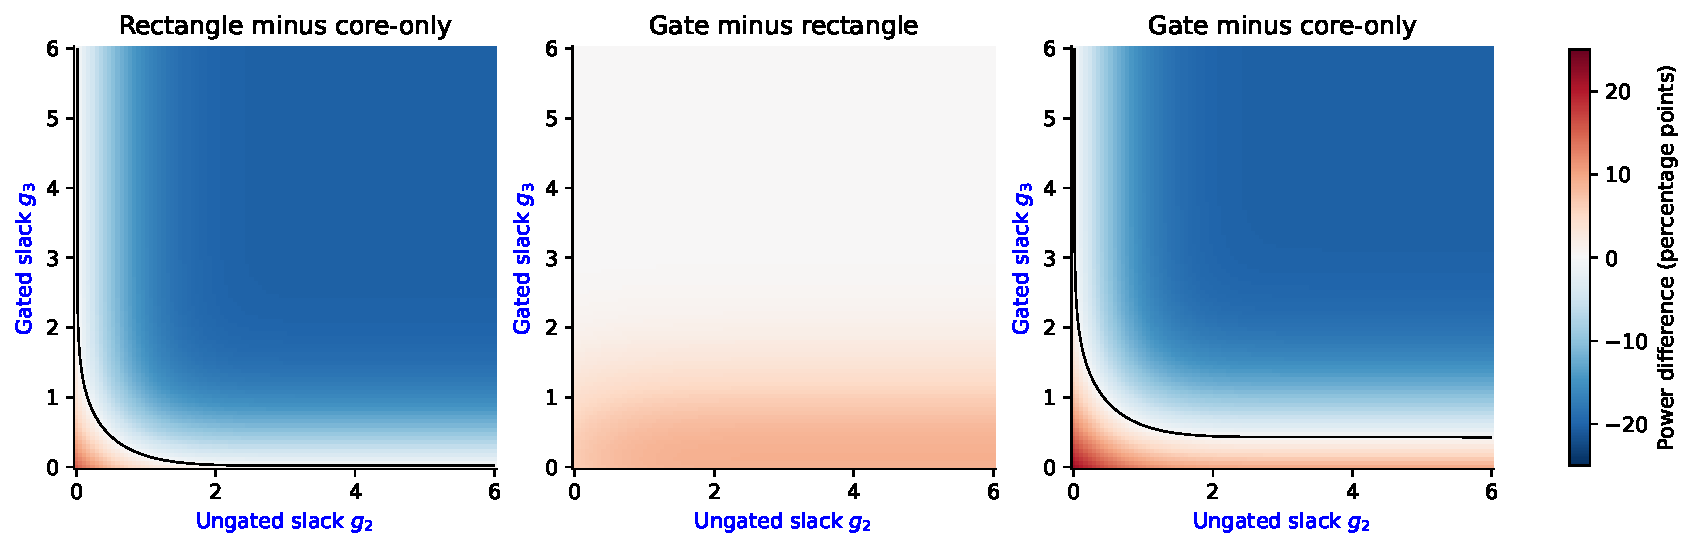
\includegraphics[width=\textwidth]{figures/sec4-pilot-gate.pdf}
\caption{Differences in power, in percentage points, with one core inequality at $\delta=(s,\ s-g_2,\ s-g_3)'$ and $s=c_1$, so that the core-only test has power $50\%$. The gate pairs coordinates 1 and 3. Independent moments with a common scale, $\alpha=0.10$. The black curves mark a difference of zero.}
\label{fig:gate}
\end{figure}

The gate improves on the rectangle everywhere, as Theorem~\ref{thm:gate} requires, but by an amount that depends on the paired coordinate. At this value of $s$, the improvement reaches about $9.0$ points, and it is $8.9$ points at $(g_2,g_3)=(3,0)$. When the paired inequality is slack, it nearly vanishes, and at $(g_2,g_3)=(0,3)$ it is $0.1$ points. The rectangle has the same power at these two alternatives and the gate does not, because the pairing is fixed. This illustrates how a strict improvement at every alternative need not be a large one.

Dropping the redundant inequalities gives a different comparison. The rectangle gains the most over the core-only test when both redundant inequalities are violated by as much as the core inequality, where the gain is $15.1$ points. A gain does not require both to be close to the core inequality: at $(g_2,g_3)=(3,0)$ it is still positive, at $0.4$ points. Along the diagonal $g_2=g_3$, the gain turns into a loss once the common slack exceeds approximately $0.47$, and when both redundant inequalities are slack by three standard deviations the rectangle loses $20.4$ points, which is approximately the price of using $c_3$ in place of $c_1$.

The gate improves on the rectangle but does not remove this trade-off with the core-only test. It gains $21.3$ points when $g_2=g_3=0$ and $9.3$ points at $(g_2,g_3)=(3,0)$, but it loses $20.3$ points at $(g_2,g_3)=(3,3)$, where the redundant inequalities contribute little beyond a larger cutoff.

We can also compare the three tests by minimax regret. Since the gate dominates the rectangle, the highest power at each alternative is attained by either the gate or the core-only test. We measure each test's regret relative to this benchmark. Table~\ref{tab:one-core-regret} reports the largest regrets over all $s>0$ and $g_2,g_3\ge0$, allowing the core signal to vary as well.

\begin{table}[!ht]
\centering

\begin{tabular}{lc}
\toprule
Test & Maximum regret\\
\midrule
Core-only & 22.93\\
Rectangle & 21.16\\
Gate on $(1,3)$ & 21.16\\
\bottomrule
\end{tabular}
\caption{Maximum regret, in percentage points, relative to the most powerful of the three tests at each alternative. One core inequality, independent moments with a common scale, $\alpha=0.10$. Suprema are taken over the full one-core alternative.}
\label{tab:one-core-regret}
\end{table}

For this design, retaining has a modest advantage under minimax regret, which does not distinguish the gate from the rectangle. Their largest regrets are approached when both redundant means become arbitrarily negative. In that limit, both tests reject only when $X_1>c_3$, and their power loss relative to the core-only test is the same. The gate improves on the rectangle at every alternative, but that improvement vanishes along the alternatives that determine maximum regret. In this example, minimax regret therefore does not distinguish the rectangle from a test that uniformly improves upon it.

The gate's improvement still depends on knowing which core bounds the redundant means. In the two-core model, at $\delta=(-6,1,1)'$, the rectangle has power $37.1\%$ and the gate $20.7\%$, a loss of $16.4$ points. Here $\delta_2$ bounds $\delta_3$ while $\delta_1$ is far below zero, so pairing $X_3$ with $X_1$ gives up rejections that the rectangle keeps, as in Section~\ref{sec:three-moments}.

The comparisons above impose the standardized ordering of Section~\ref{sec:normal}, which prevents a redundant inequality from having a larger signal than every core inequality. Appendix~\ref{app:precision} considers an ordering in the original units and varies the precision of the redundant moment. Greater precision can substantially increase the cost of dropping it, while leaving the largest cost of keeping it unchanged.

% Placeholder (not in the PDF): finite-sample evidence. The simulations in R2-D2's plan (studentization,
% moment selection, size) have not been run. Add a short subsection here only if the results qualify the
% Gaussian comparisons above; otherwise report them in a supplement.


%%%%%%%%% -------------------------------------------------------------------
\section{Concluding Remarks}\label{sec:conclusions}
%%%%%%%%% -------------------------------------------------------------------


\newpage 
%%%%%%%%% -------------------------------------------------------------------
\appendices
%%%%%%%%% -------------------------------------------------------------------

\renewcommand{\theequation}{\Alph{section}-\arabic{equation}}
\setcounter{equation}{0}

\section{Proofs for Section \ref{sec:normal}}\label{app:proofs-normal}

% Proofs ported from notes/general-case.tex (August 28, 2026), with notation adapted to the paper.
% The proof of the two-moment theorem (Appendix A.11) is ported from notes/necessity-feasible-normal-general-omega.tex.

Throughout, $P_\mu$ denotes the distribution of $X\sim N_d(\mu,\Omega)$ and, for a test $\psi$, $h:=\psi-\phi$ with $h=h^+-h^-$. Relative to $P_0$, the likelihood ratio is
\begin{equation}\label{eq:lr}
\frac{dP_\mu}{dP_0}(x)=\exp\Big\{\mu'\Omega^{-1}x-\frac12\,\mu'\Omega^{-1}\mu\Big\}~.
\end{equation}

\subsection{Proof of Lemma \ref{lem:dual}}

Suppose first that $\mathcal C=\{1\}$. Every $\mu\in\Lambda_1$ has $\mu_1>0$, and since $\Lambda_1$ is a cone we may normalize $\mu_1=1$. The condition $v\in\Lambda_1^*$ then reads
\[
v_1+\sum_{r\in\mathcal R}\mu_rv_r\ge0
\qquad\text{for every }(\mu_r)_{r\in\mathcal R}\text{ with }\mu_r\le1~.
\]
Sending one $\mu_r$ to $-\infty$ shows that $v_r\le0$. Given these signs, the left side is smallest when $\mu_r=1$ for every $r$, which gives $v_1+\sum_rv_r\ge0$. The two conditions are also sufficient. The representation as a cone follows from
\[
v=\Big(v_1+\sum_{r\in\mathcal R}v_r\Big)e_1+\sum_{r\in\mathcal R}(-v_r)(e_1-e_r)~.
\]

Now suppose that $|\mathcal C|\ge2$ and $v\in\Lambda_1^*$. Fix $j\in\mathcal C$ and choose $c\in\mathcal C$ with $c\ne j$. For every $s\in\mathbf R$, the mean $e_c+se_j$ belongs to $\Lambda_1$, so $v_c+sv_j\ge0$ for every $s\in\mathbf R$, which forces $v_j=0$. For $r\in\mathcal R$, the mean $e_c+se_r$ belongs to $\Lambda_1$ for every $s\le1$, so $sv_r\ge0$ for every $s\le1$. Taking $s=1$ and $s=-1$ gives $v_r=0$. \qed

\subsection{Proof of Lemma \ref{lem:first-order}}

Level control gives $E_0[h(X)]\le0$. For $c\in\mathcal C$ and $t>0$, $te_c\in\Lambda_1$, and dominance together with continuity of $t\mapsto E_{te_c}[h(X)]$ at zero gives $E_0[h(X)]\ge0$. Hence $E_0[h(X)]=0$.

Fix $\mu\in\Lambda_1$. Since $\Lambda_1$ is a cone, $f(t):=E_{t\mu}[h(X)]\ge0$ for every $t>0$, and $f(0)=0$. Because $|h|\le1$ and the Gaussian moment-generating function is finite, we may differentiate under the expectation, and \eqref{eq:lr} gives
\[
0\le f'(0+)=\mu'\Omega^{-1}E_0[Xh(X)]~.
\]
Thus $\Omega^{-1}E_0[Xh(X)]\in\Lambda_1^*$. When $|\mathcal C|\ge2$, Lemma~\ref{lem:dual}(b) gives $\Omega^{-1}E_0[Xh(X)]=0$, and nonsingularity of $\Omega$ gives $E_0[Xh(X)]=0$. \qed

\subsection{An auxiliary lemma}

\begin{lemma}\label{lem:feasible-alternative}
If $a\in\mathcal F(\Omega,\Lambda)$ and $a\ne0$, then $\Omega a\in\Lambda_1$.
\end{lemma}

\begin{proof}
Suppose instead that every core component of $\Omega a$ is nonpositive. Because $\Omega a\in\Lambda$, every redundant component is then nonpositive as well. Since $a\ge0$, this implies $a'\Omega a\le0$, which contradicts positive definiteness.
\end{proof}

\subsection{Proof of Proposition \ref{prop:feasible-support}}

Let $\psi$ be a level-$\alpha$ test that weakly dominates $\phi_A$ and set $h:=\psi-\phi_A$. As in the proof of Lemma~\ref{lem:first-order}, $E_0[h(X)]=0$. Moreover,
\begin{equation}\label{eq:signs}
\{h>0\}\subseteq A~,
\qquad
\{h<0\}\subseteq A^c~.
\end{equation}
Fix $a\in F_A$. By Lemma~\ref{lem:feasible-alternative}, $t\Omega a\in\Lambda_1$ for every $t>0$, so dominance and \eqref{eq:lr} give
\begin{equation}\label{eq:tilt}
E_0\big[e^{ta'X}h(X)\big]\ge0
\qquad\text{for every }t>0~.
\end{equation}
Since $h^+$ is supported on $A\subseteq\{x:\ a'x\le h_A(a)\}$, for every $\varepsilon>0$,
\[
E_0\big[e^{ta'X}h(X)\big]
\le e^{th_A(a)}E_0[h^+(X)]
-e^{t\{h_A(a)+\varepsilon\}}E_0\big[h^-(X)I\{a'X\ge h_A(a)+\varepsilon\}\big]~.
\]
If the last expectation were positive, the right side would be negative for all sufficiently large $t$, which contradicts \eqref{eq:tilt}. Taking $\varepsilon=1/n$ for $n\ge1$ shows that $h^-=0$ almost surely on $\{x:\ a'x>h_A(a)\}$.

By feasible support, the open set $A^c$ is the union of the open halfspaces $\{x:\ a'x>h_A(a)\}$ over $a\in F_A$, and a countable subfamily covers it. Hence $h^-=0$ almost surely on $A^c$, and \eqref{eq:signs} gives $h^-=0$ almost surely. Since $E_0[h(X)]=0$, also $h^+=0$ almost surely. Gaussian shifts are mutually absolutely continuous, so $\psi=\phi_A$ almost surely under every $P_\mu$, and no strict improvement is possible. \qed

\subsection{Proof of Proposition \ref{prop:relation}}

The first statement follows from the representation of a closed convex set as the intersection of its supporting halfspaces. Suppose now that $|\mathcal C|=1$. Then $\Lambda$ is defined by finitely many linear inequalities, so $\mathcal F(\Omega,\Lambda)$ is a closed convex cone. Let $A$ be feasibly supported and let $b$ be a finite normal of $A$. If $b\notin\mathcal F(\Omega,\Lambda)$, a separating hyperplane gives $v\in\mathbf R^d$ with
\[
a'v\le0\ \text{ for every }a\in\mathcal F(\Omega,\Lambda)~,
\qquad
b'v>0~.
\]
For $x\in A$ and $t\ge0$, every halfspace in Definition~\ref{def:feasible-support} contains $x+tv$, so feasible support gives $x+tv\in A$. Then $h_A(b)\ge b'x+tb'v\to\infty$, a contradiction. \qed

\subsection{Proof of Corollary \ref{cor:core-only}}

The facets of $A_{\mathcal C}$ have normals $e_c$, $c\in\mathcal C$. For $r\in\mathcal R$, $(\Omega e_c)_r=\Omega_{rc}<1=(\Omega e_c)_c$, where the strict inequality uses positive definiteness and the unit diagonal. Hence $\Omega e_c\in\Lambda$, every facet normal is feasible, and Proposition~\ref{prop:feasible-support} applies. \qed

\subsection{Proof of Theorem \ref{thm:one-extra}}

Let $\psi$ be a level-$\alpha$ test that weakly dominates $\phi_A$ and set $h:=\psi-\phi_A$. Lemma~\ref{lem:first-order} gives
\begin{equation}\label{eq:balance}
E_0[h(X)]=0~,
\qquad
E_0[Xh(X)]=0~.
\end{equation}
For every $a\in G$, the argument in the proof of Proposition~\ref{prop:feasible-support}, with $\kappa_a$ in place of $h_A(a)$, shows that $h^-=0$ almost surely on $\{x:\ a'x>\kappa_a\}$. A countable subfamily covers $A_f^c$, so $h^-=0$ almost surely on $A_f^c$. Since $h^-$ is supported on $A^c$, any remaining negative part is supported on $A_f\cap\{x:\ u'x>\kappa\}$, while $h^+$ is supported on $A\subseteq\{x:\ u'x\le\kappa\}$.

Let $M:=E_0[h^+(X)]=E_0[h^-(X)]$, where the equality follows from \eqref{eq:balance}. If $M>0$, then
\[
E_0[u'Xh^+(X)]\le\kappa M~,
\qquad
E_0[u'Xh^-(X)]>\kappa M~,
\]
where the second inequality is strict because $u'X>\kappa$ on the support of $h^-$ and $u'X$ has no atom at $\kappa$. Then $u'E_0[Xh(X)]<0$, which contradicts \eqref{eq:balance}. Hence $M=0$, so $h=0$ almost surely, and mutual absolute continuity rules out a strict improvement. \qed

\subsection{Proofs of Corollaries \ref{cor:halfspace} and \ref{cor:rectangles}}

For Corollary~\ref{cor:halfspace}, the acceptance region $\{x:\ a'x\le z_{1-\alpha}\sqrt{a'\Omega a}\}$ is nice. Apply Theorem~\ref{thm:one-extra} with $A_f=\mathbf R^d$ and $u=a$.

For Corollary~\ref{cor:rectangles}, write $\mathcal R=\{r\}$. As in the proof of Corollary~\ref{cor:core-only}, every core face has a feasible normal. The redundant face $\{x:\ x_r\le\kappa_r\}$ is the one arbitrary halfspace, and Theorem~\ref{thm:one-extra} applies. \qed

\subsection{Proof of Corollary \ref{cor:epsilon}}

At $\varepsilon=0$, $(\Omega e_1)_1=1$ and $(\Omega e_1)_r=\Omega_{r1}<1$ for every $r\in\mathcal R$. By continuity and finiteness of $\mathcal R$, $(\Omega a_\varepsilon)_r<(\Omega a_\varepsilon)_1$ for every $r\in\mathcal R$ and all sufficiently small $\varepsilon>0$. Since $a_\varepsilon\ge0$, this gives $a_\varepsilon\in\mathcal F(\Omega,\Lambda)$. The acceptance region is a halfspace with this single feasible normal, so it is feasibly supported, and Proposition~\ref{prop:feasible-support} applies. \qed

\subsection{Proof of Theorem \ref{thm:gate}}

The left side of \eqref{eq:gate-calibration} is continuous and strictly increasing in $b_r$, from $0$ to $\Phi(\kappa_1)$, and the right side lies strictly between these limits, so $b_r$ exists and is unique. Independence and \eqref{eq:gate-calibration} give $P_0\{X\in A_\kappa^{(r)}\}=P_0\{X\in A_\kappa\}=1-\alpha$, and $A_\kappa^{(r)}$ is lower, so the gated test has level $\alpha$.

In the coordinates $(x_1,x_r)$, the points rejected by the gated test and accepted by the rectangle, and the points accepted by the gated test and rejected by the rectangle, are
\[
G_r:=\{x_1\le\kappa_1,\ x_r\le\kappa_r,\ x_1+x_r>b_r\}~,
\qquad
D_r:=\{x_1\le\kappa_1,\ x_r>\kappa_r,\ x_1+x_r\le b_r\}~.
\]
Calibration gives $P_0(G_r)=P_0(D_r)$. This common probability is positive, since calibration forces $b_r<\kappa_1+\kappa_r$. Every $g\in G_r$ and $d\in D_r$ satisfy
\[
g_1+g_r>d_1+d_r~,
\qquad
-g_r>-d_r~.
\]
For $\mu\in\Lambda_1$, let $u:=\mu_1>0$ and $v:=\mu_1-\mu_r\ge0$, and set $\ell(x):=u(x_1+x_r)-vx_r$ and $L:=ub_r-v\kappa_r$. Then $\ell(g)>L$ for every $g\in G_r$ and $\ell(d)\le L$ for every $d\in D_r$. Since the likelihood ratio in the coordinates $(x_1,x_r)$ is proportional to $e^{\ell(x)}$,
\[
\int_{G_r}e^{\ell(x)}\,dP_0(x)>e^{L}P_0(G_r)=e^{L}P_0(D_r)\ge\int_{D_r}e^{\ell(x)}\,dP_0(x)~,
\]
so $P_\mu(G_r)>P_\mu(D_r)$. The remaining rectangular constraints are independent of $(X_1,X_r)$ and common to both tests, and they contribute the positive factor $\prod_{j\notin\{1,r\}}\Phi(\kappa_j-\mu_j)$. Hence the gated test is strictly more powerful at every $\mu\in\Lambda_1$. In terms of Lemma~\ref{lem:dual}, with $w:=g-d$ in the coordinates $(x_1,x_r)$, the move from a removed point to an added point is $w=(w_1+w_r)e_1+(-w_r)(e_1-e_r)$, and both coefficients are positive. \qed

\subsection{Proof of Theorem \ref{thm:two-moments}}\label{app:proof-two-moments}

% Ported from notes/necessity-feasible-normal-general-omega.tex (August 27, 2026), notation adapted to the paper.

Throughout this subsection, $d=2$, $\mathcal C=\{1\}$, $\mathcal R=\{2\}$, $\Omega=\Omega_\rho$ with $-1<\rho<1$, and $\Lambda=\{\mu:\mu_2\le\mu_1\}$, so that $\Lambda_1=\{\mu\in\Lambda:\mu_1>0\}$ and $\mathcal F_\rho:=\mathcal F(\Omega_\rho,\Lambda)=\{a:0\le a_2\le a_1\}$. Let $A$ be a nice region, and write $P_0(C):=P_0\{X\in C\}$ for a Borel set $C$.

\emph{Sufficiency.} If every finite normal of $A$ lies in $\mathcal F_\rho$, then $A$ is feasibly supported by Proposition~\ref{prop:relation}, and $\phi_A$ is $\alpha$-admissible by Proposition~\ref{prop:feasible-support}.

\emph{Necessity.} Since $A$ is lower, every finite normal is nonnegative. If the condition fails, there is therefore $a\ne0$ with $h_A(a)<\infty$ and $0\le a_1<a_2$. Lemma~\ref{lem:bv-necessity} below constructs a level-$\alpha$ test that strictly dominates $\phi_A$ at every $\mu\in\Lambda_1$, so $\phi_A$ is inadmissible. The rest of this subsection proves that lemma.

\subsubsection*{The transfer order}

Let $\mathbf 1:=(1,1)'$ and define the scores
\[
T_{1,\rho}(x):=(\Omega_\rho^{-1}\mathbf 1)'x=\frac{x_1+x_2}{1+\rho}~,
\qquad
T_{2,\rho}(x):=-(\Omega_\rho^{-1}e_2)'x=\frac{\rho x_1-x_2}{1-\rho^2}~.
\]
The cone of moves that raise both scores is
\begin{equation}\label{eq:bv-transfer-cone}
\Pi_\rho:=\{p:\ T_{1,\rho}(p)\ge0,\ T_{2,\rho}(p)\ge0\}
=\operatorname{cone}\{(1,\rho),(1,-1)\}
=\{p:\ p_1+p_2\ge0,\ \rho p_1-p_2\ge0\}~.
\end{equation}
The direction $(1,\rho)$ raises $T_{1,\rho}$ and leaves $T_{2,\rho}$ unchanged, and the direction $(1,-1)$ raises $T_{2,\rho}$ and leaves $T_{1,\rho}$ unchanged. For $\mu\in\Lambda_1$, write $u:=\mu_1>0$ and $v:=\mu_1-\mu_2\ge0$, so that $\mu=u\mathbf 1-ve_2$. Then
\begin{equation}\label{eq:bv-LR}
L_\mu(x):=\frac{dP_\mu}{dP_0}(x)=\exp\Big\{uT_{1,\rho}(x)+vT_{2,\rho}(x)-\frac12\,\mu'\Omega_\rho^{-1}\mu\Big\}~,
\end{equation}
which is strictly increasing in $T_{1,\rho}$ and weakly increasing in $T_{2,\rho}$.

The competitor starts from the closed hull
\[
\widehat A_\rho:=\operatorname{cl}(A-\Pi_\rho)~,
\]
the smallest closed set that contains $A$ and is closed under moves opposite to $\Pi_\rho$. This operation removes boundary pieces with infeasible normals. It also adds acceptance probability, which the competitor restores by cutting $\widehat A_\rho$ with a halfspace in $T_{1,\rho}$.

\begin{lemma}\label{lem:bv-hull}
The set $\widehat A_\rho$ is closed, convex, lower, and $\Pi_\rho$-lower, that is, $x\in\widehat A_\rho$ and $p\in\Pi_\rho$ imply $x-p\in\widehat A_\rho$. Every finite normal of $\widehat A_\rho$ lies in $\mathcal F_\rho$. If $A$ has a finite normal $a$ with $a_2>a_1$, then $A\subsetneq\widehat A_\rho$ and $P_0(\widehat A_\rho)>P_0(A)$.
\end{lemma}

\begin{proof}
As the closure of the Minkowski sum $A+(-\Pi_\rho)$, the set $\widehat A_\rho$ is closed and convex, and it contains $A$ because $0\in\Pi_\rho$. It is lower: if $x=y-p$ with $y\in A$ and $p\in\Pi_\rho$, and $z\le x$, then $z=(y-(x-z))-p$ with $y-(x-z)\in A$; passing to the closure preserves this property. The $\Pi_\rho$-lower property follows from the definition.

The support function satisfies $h_{\widehat A_\rho}(a)=h_A(a)+h_{-\Pi_\rho}(a)$. Since $-\Pi_\rho$ is generated by $(-1,-\rho)$ and $(-1,1)$,
\begin{equation}\label{eq:bv-polar}
h_{-\Pi_\rho}(a)<\infty
\quad\Longleftrightarrow\quad
a_1+\rho a_2\ge0
\ \text{ and }\
a_2\le a_1~.
\end{equation}
Since $A$ is lower and nonempty, $h_A(a)<\infty$ implies $a\ge0$. Hence a finite normal of $\widehat A_\rho$ satisfies $a\ge0$ and $a_2\le a_1$, so $a\in\mathcal F_\rho$. (The first inequality in \eqref{eq:bv-polar} is then automatic: it is immediate for $\rho\ge0$, and for $\rho<0$, $a_1+\rho a_2\ge(1+\rho)a_1\ge0$.)

Now suppose $h_A(a)<\infty$ for some $a$ with $a_2>a_1$. Every $x\in A$ generates the ray $x+t(-1,1)\in A-\Pi_\rho$, $t\ge0$, along which $a'\{x+t(-1,1)\}=a'x+t(a_2-a_1)\to\infty$. Hence $\widehat A_\rho$ is not contained in the supporting halfspace $\{x:\ a'x\le h_A(a)\}$, and $\widehat A_\rho\setminus A$ is nonempty. Since $P_0(A)\in(0,1)$ and $A$ is convex, $A$ has nonempty interior. Joining a point of $\widehat A_\rho$ outside that halfspace to an interior point of $A$ gives a nonempty open subset of $\widehat A_\rho\setminus A$. The Gaussian density is positive everywhere, so $P_0(\widehat A_\rho)>P_0(A)$.
\end{proof}

\begin{lemma}\label{lem:bv-competitor}
Suppose that $A$ has a finite normal $a$ with $a_2>a_1$. Then there is a finite $b$ such that
\[
A':=\widehat A_\rho\cap\{x:\ T_{1,\rho}(x)\le b\}
\]
satisfies $P_0(A')=1-\alpha$. The set $A'$ is closed, convex, lower, and $\Pi_\rho$-lower, every finite normal of $A'$ lies in $\mathcal F_\rho$, and $\phi_{A'}$ is a level-$\alpha$ test with size attained at the origin.
\end{lemma}

\begin{proof}
By Lemma~\ref{lem:bv-hull}, $P_0(\widehat A_\rho)>1-\alpha$. The map $t\mapsto P_0(\widehat A_\rho\cap\{T_{1,\rho}\le t\})$ is continuous, because $T_{1,\rho}(X)$ is nondegenerate normal under $P_0$, and it increases from $0$ to $P_0(\widehat A_\rho)$. Hence a finite $b$ with the stated property exists.

The set $A'$ is closed and convex, and it is lower because $T_{1,\rho}$ is increasing in each coordinate ($1+\rho>0$). It is $\Pi_\rho$-lower: if $x\in A'$ and $p\in\Pi_\rho$, then $x-p\in\widehat A_\rho$ by Lemma~\ref{lem:bv-hull}, and $T_{1,\rho}(x-p)=T_{1,\rho}(x)-T_{1,\rho}(p)\le b$.

Let $a\ne0$ be a finite normal of $A'$ and fix $x\in A'$. Lowerness gives $a\ge0$, as in Lemma~\ref{lem:bv-hull}. Since $(1,-1)\in\Pi_\rho$, $x-t(1,-1)\in A'$ for every $t\ge0$, and $a'\{x-t(1,-1)\}=a'x+t(a_2-a_1)$. Finite support therefore forces $a_2\le a_1$, so $a\in\mathcal F_\rho$.

Finally, the complement of $A'$ is upper, and every $\mu\in\Lambda_0$ satisfies $\mu\le0$. Writing $X=\mu+Z$ with $Z\sim N_2(0,\Omega_\rho)$ gives $P_\mu\{X\notin A'\}\le P_0\{Z\notin A'\}=\alpha$, with equality at $\mu=0$.
\end{proof}

\begin{lemma}\label{lem:bv-transfer}
Let $G$ and $D$ be Borel sets with $P_0(G)=P_0(D)>0$, and suppose that every $g\in G$ and $d\in D$ satisfy $T_{1,\rho}(g)>T_{1,\rho}(d)$ and $T_{2,\rho}(g)\ge T_{2,\rho}(d)$. Then $P_\mu(G)>P_\mu(D)$ for every $\mu\in\Lambda_1$.
\end{lemma}

\begin{proof}
Let $m:=P_0(G)=P_0(D)$. By \eqref{eq:bv-LR},
\[
m\{P_\mu(G)-P_\mu(D)\}=\int_G\int_D\{L_\mu(g)-L_\mu(d)\}\,dP_0(d)\,dP_0(g)~.
\]
For $\mu\in\Lambda_1$, the coefficient on $T_{1,\rho}$ in \eqref{eq:bv-LR} is $u>0$ and the coefficient on $T_{2,\rho}$ is $v\ge0$, so $L_\mu(g)>L_\mu(d)$ for every pair $(g,d)\in G\times D$. Since $m>0$, the double integral is positive.
\end{proof}

\subsubsection*{Slices and the two cases}

Although $\Pi_\rho$ depends on $\rho$, the hull does not. Let $K:=\operatorname{cone}\{(1,-1)\}$. If $\rho\ge0$, subtracting a nonnegative multiple of $(1,\rho)$ is a coordinatewise downward move and is absorbed by $A$. If $\rho<0$, then $(1,\rho)=(-\rho)(1,-1)+(1+\rho)e_1$ with both coefficients positive, and subtracting the second term is again a downward move. In both cases,
\begin{equation}\label{eq:bv-hull-reduction}
A-\Pi_\rho=A-K~,
\qquad
\widehat A_\rho=\operatorname{cl}(A-K)~.
\end{equation}
For $s\in\mathbf R$, let $\beta(s):=\sup\{x_1:(x_1,s)\in A\}\in[-\infty,\infty]$. Since $A$ is closed, convex, and lower, $A\cap\{x_2=s\}=\{(x_1,s):x_1\le\beta(s)\}$, and $\beta$ is concave in the extended-real sense. Set
\[
m(s):=\beta(s)+s~,
\qquad
M(s):=\sup_{r\le s}m(r)~.
\]
Thus $m(s)$ is the largest value of $x_1+x_2=(1+\rho)T_{1,\rho}(x)$ on the horizontal slice of $A$ at height $s$, and $M(s)$ is its running maximum from below.

\begin{lemma}\label{lem:bv-slice}
For every $s\in\mathbf R$, $(x_1,s)\in\widehat A_\rho$ if and only if $x_1+s\le M(s)$.
\end{lemma}

\begin{proof}
Let $C:=\{(x_1,s):x_1+s\le M(s)\}$. We first show that $C$ is closed. The function $M$ never equals $-\infty$: fix $(x_1^0,s_0)\in A$; if $s\ge s_0$, then $M(s)\ge m(s_0)>-\infty$, and if $s<s_0$, lowerness gives $(x_1^0,s)\in A$, so $M(s)\ge m(s)>-\infty$. The function $M$ is nondecreasing, and it is concave where finite: for $s_1,s_2$ and $\varepsilon>0$, choose $r_i\le s_i$ with $m(r_i)\ge M(s_i)-\varepsilon$; for $\lambda\in[0,1]$, concavity of $m$ gives
\[
M\{\lambda s_1+(1-\lambda)s_2\}\ge m\{\lambda r_1+(1-\lambda)r_2\}\ge\lambda M(s_1)+(1-\lambda)M(s_2)-\varepsilon~.
\]
If $M(s_0)=\infty$ for some $s_0$, then $M\equiv\infty$. Monotonicity gives this to the right of $s_0$. For $t<s_0$, choose $r_n\le s_0$ with $m(r_n)\to\infty$. If $r_n\le t$ along a subsequence, then $M(t)=\infty$. Otherwise $t<r_n\le s_0$ eventually, and lowerness gives $\beta(t)\ge\beta(r_n)$, so $m(t)\ge m(r_n)+t-s_0\to\infty$. Hence either $M\equiv\infty$ and $C=\mathbf R^2$, or $M$ is a finite concave, hence continuous, function. In both cases $C$ is closed.

If $(x_1,s)\in A-K$, then by \eqref{eq:bv-hull-reduction} there are $(y_1,r)\in A$ and $\tau\ge0$ with $(x_1,s)=(y_1,r)-\tau(1,-1)$. Then $r=s-\tau\le s$ and $x_1+s=y_1+r\le m(r)\le M(s)$. Thus $A-K\subseteq C$, and closedness of $C$ gives $\widehat A_\rho\subseteq C$.

Conversely, suppose $x_1+s<M(s)$. Then there is $r\le s$ with $m(r)>x_1+s$, and hence $y_1\le\beta(r)$ with $(y_1,r)\in A$ and $y_1+r>x_1+s$. By lowerness, $(\widetilde y_1,r)\in A$ for $\widetilde y_1:=x_1+s-r<y_1$, and with $\tau:=s-r\ge0$ we obtain $(x_1,s)=(\widetilde y_1,r)-\tau(1,-1)\in A-K$. If $x_1+s=M(s)$, apply this argument to $(x_1-1/n,s)$ and let $n\to\infty$; since $\widehat A_\rho$ is closed, $(x_1,s)\in\widehat A_\rho$.
\end{proof}

For $\rho<0$, let $q_\rho:=(1,\rho)$, and call a set $C$ \emph{$q_\rho$-lower} if $x\in C$ and $t\ge0$ imply $x-tq_\rho\in C$. When $\rho\ge0$, every lower set has this property. When $\rho<0$, it is an additional restriction, because subtracting $q_\rho$ lowers the first coordinate and raises the second. The next two lemmas treat the two possibilities.

\begin{lemma}\label{lem:bv-rearrangement}
Suppose $\rho<0$ and $A$ is not $q_\rho$-lower. Then there is a Borel set $A^{\mathrm r}$ such that $\phi_{A^{\mathrm r}}$ is a level-$\alpha$ test and $P_\mu(A^{\mathrm r})<P_\mu(A)$ for every $\mu\in\Lambda_1$. In particular, $\phi_{A^{\mathrm r}}$ strictly dominates $\phi_A$.
\end{lemma}

\begin{proof}
Let $Z:=X_1$ and $E:=X_2-\rho X_1$. Writing $\mu=(u,u-v)$ with $v\ge0$ on $\Lambda$, we have
\[
Z\sim N(u,1)~,
\qquad
E\sim N\big((1-\rho)u-v,\ 1-\rho^2\big)~,
\qquad
Z\perp E~.
\]
Let $\gamma$ denote the standard normal distribution on $\mathbf R$. For $e\in\mathbf R$, let $A_e:=\{z:(z,e+\rho z)\in A\}$ and $p(e):=\gamma(A_e)$. By Fubini's theorem, $p$ is measurable. If $e_1\le e_2$, lowerness of $A$ gives $A_{e_2}\subseteq A_{e_1}$, so $p$ is nonincreasing. Let $c(e):=\Phi^{-1}\{p(e)\}$, with $c(e)=-\infty$ when $p(e)=0$ and $c(e)=\infty$ when $p(e)=1$, and define
\[
A^{\mathrm r}:=\{x:\ x_1\le c(x_2-\rho x_1)\}~.
\]
The function $c$ is measurable and nonincreasing, so in the coordinates $(z,e)$ the set $A^{\mathrm r}=\{(z,e):z\le c(e)\}$ is Borel and lower.

Under $P_0$, $Z$ and $E$ are independent and each section keeps its standard normal mass, so $P_0(A^{\mathrm r})=P_0(A)=1-\alpha$. If $\mu\in\Lambda_0$, then $u\le0$ and $v\ge0$, so $(u,(1-\rho)u-v)\le(0,0)$. Since $A^{\mathrm r}$ is lower in $(z,e)$, translation gives $P_\mu(A^{\mathrm r})\ge P_0(A^{\mathrm r})=1-\alpha$, so $\phi_{A^{\mathrm r}}$ has level $\alpha$, with size attained at the origin.

Now fix $\mu\in\Lambda_1$, so that $u>0$. Conditional on $E=e$, the likelihood ratio of $N(u,1)$ relative to $N(0,1)$ is strictly increasing in $z$. Among all subsets of $\mathbf R$ with standard normal probability $p(e)$, the halfline $(-\infty,c(e)]$ therefore has the smallest $N(u,1)$ probability. Integrating over $E$ gives
\begin{equation}\label{eq:bv-weak-rearrangement}
P_\mu(A^{\mathrm r})\le P_\mu(A)~.
\end{equation}

For strictness, since $A$ is not $q_\rho$-lower, there are $x\in A$ and $t>0$ with $x-tq_\rho\notin A$. As $A$ has nonempty interior, we may move $x$ slightly toward an interior point to obtain $x^0\in\operatorname{int}(A)$ and $t_0>0$ with $x^0-t_0q_\rho\notin A$. Since $A$ is closed, there are small open neighborhoods of these two points, the first contained in $A$ and the second in its complement. Under the invertible map $H(x):=(x_1,x_2-\rho x_1)$, the two centers have the same second coordinate, and their first coordinates differ by $t_0$. The images of the neighborhoods therefore contain two rectangles with a common interval of values of $e$. For every $e$ in a smaller such interval, $A_e$ contains an interval lying strictly to the right of an interval it omits, so $A_e$ is not a left halfline up to a $\gamma$-null set, and the conditional inequality is strict. Since $E$ has a positive density, integration makes \eqref{eq:bv-weak-rearrangement} strict for every $\mu\in\Lambda_1$.
\end{proof}

\begin{lemma}\label{lem:bv-gain-loss}
Suppose that $A$ has a finite normal $a$ with $a_2>a_1$, and let $A'$ and $b$ be as in Lemma~\ref{lem:bv-competitor}. Let
\[
G:=A\setminus A'=A\cap\{T_{1,\rho}>b\}~,
\qquad
D:=A'\setminus A~.
\]
Suppose either that $0\le\rho<1$, or that $-1<\rho<0$ and $A$ is $q_\rho$-lower. Then $P_0(G)=P_0(D)>0$, and every $g\in G$ and $d\in D$ satisfy $T_{1,\rho}(g)>T_{1,\rho}(d)$ and $T_{2,\rho}(g)\ge T_{2,\rho}(d)$.
\end{lemma}

\begin{proof}
Since $A\subseteq\widehat A_\rho$, we have $A\setminus A'=A\cap\{T_{1,\rho}>b\}$, and $P_0(A)=P_0(A')=1-\alpha$ gives $P_0(G)=P_0(D)$. This common mass is positive. Otherwise $A$ and $A'$ would differ by a Gaussian null set. Both are closed and convex with nonempty interior, so joining a point of one set outside the other to an interior point of the first would produce a nonempty open subset of their symmetric difference, which has positive probability. Hence $A=A'$, which is impossible because every finite normal of $A'$ lies in $\mathcal F_\rho$ (Lemma~\ref{lem:bv-competitor}) and $A$ has one outside it.

Let $B_\rho:=(1+\rho)b$, so that $T_{1,\rho}(x)\le b$ if and only if $x_1+x_2\le B_\rho$. On the slice $x_2=s$, the gain set is $G_s:=\{x_1:(x_1,s)\in G\}=(B_\rho-s,\beta(s)]$, so
\begin{equation}\label{eq:bv-gain-slice}
G_s\ne\varnothing
\quad\Longleftrightarrow\quad
m(s)>B_\rho~.
\end{equation}
By Lemma~\ref{lem:bv-slice}, the loss slice is $D_s:=\{x_1:(x_1,s)\in D\}=(\beta(s),\min\{M(s),B_\rho\}-s]$, so
\begin{equation}\label{eq:bv-loss-slice}
D_s\ne\varnothing
\quad\Longleftrightarrow\quad
M(s)>m(s)\ \text{ and }\ m(s)<B_\rho~.
\end{equation}
Let $s_+:=\sup\{s:m(s)>B_\rho\}$, which is well defined because $P_0(G)>0$. By \eqref{eq:bv-gain-slice}, $G_s\ne\varnothing$ implies $s\le s_+$. We claim that $D_s\ne\varnothing$ implies $s\ge s_+$. Suppose instead that $D_s\ne\varnothing$ for some $s<s_+$. By \eqref{eq:bv-loss-slice}, $M(s)>m(s)$, so there is $q<s$ with $m(q)>m(s)$. Since $s<s_+$, there is also $r>s$ with $m(r)>B_\rho>m(s)$. Writing $s=\lambda q+(1-\lambda)r$ with $\lambda\in(0,1)$, concavity of $m$ gives $m(s)\ge\lambda m(q)+(1-\lambda)m(r)>m(s)$, a contradiction. Since $D$ is nonempty, this also shows that $s_+$ is finite.

It follows that $g_2\le s_+\le d_2$ for every $g\in G$ and $d\in D$, and in fact $g_2<d_2$, because a gain slice requires $m(s)>B_\rho$ and a loss slice requires $m(s)<B_\rho$. By construction, $T_{1,\rho}(g)>b\ge T_{1,\rho}(d)$.

If $\rho\ge0$, the identity $T_{2,\rho}(x)=\{\rho T_{1,\rho}(x)-x_2\}/(1-\rho)$ gives
\[
T_{2,\rho}(g)-T_{2,\rho}(d)=\frac{\rho\{T_{1,\rho}(g)-T_{1,\rho}(d)\}+d_2-g_2}{1-\rho}\ge0~.
\]
Suppose instead that $\rho<0$ and $A$ is $q_\rho$-lower. If $s<t$ and $(x_1,s)\in A$, set $\tau:=(t-s)/(-\rho)$; then $(x_1,s)-\tau q_\rho=(x_1-\tau,t)\in A$. Hence $\beta(t)\ge\beta(s)-(t-s)/(-\rho)$ whenever these boundaries are finite, and
\begin{equation}\label{eq:bv-slope}
m(s)-m(t)\le\frac{1+\rho}{-\rho}\,(t-s)~.
\end{equation}
For $g\in G$ and $d\in D$, put $s:=g_2<t:=d_2$. The boundaries at $s$ and $t$ are finite: a gain point makes the slice at $s$ nonempty, $q_\rho$-lowerness carries such a point to height $t$, and $\beta(s)=\infty$ would force $\beta(t)=\infty$, contradicting the existence of a loss point at $t$. Therefore $g_1+s\le m(s)$ and $d_1+t>m(t)$, and \eqref{eq:bv-slope} gives
\[
(g_1+g_2)-(d_1+d_2)<\frac{1+\rho}{-\rho}\,(d_2-g_2)~.
\]
Multiplying by $\rho<0$ reverses the inequality, so
\[
(1-\rho^2)\{T_{2,\rho}(g)-T_{2,\rho}(d)\}=\rho\{(g_1+g_2)-(d_1+d_2)\}+(1+\rho)(d_2-g_2)>0~.
\]
\end{proof}

\begin{lemma}\label{lem:bv-necessity}
If $A$ has a finite normal $a$ with $a_2>a_1$, then there is a level-$\alpha$ test $\phi^*$ with $E_\mu[\phi^*(X)]>E_\mu[\phi_A(X)]$ for every $\mu\in\Lambda_1$.
\end{lemma}

\begin{proof}
Suppose first that $\rho\ge0$, and let $A'$ be as in Lemma~\ref{lem:bv-competitor}, so that $\phi_{A'}$ has level $\alpha$. With $G$ and $D$ as in Lemma~\ref{lem:bv-gain-loss},
\[
P_\mu\{X\notin A'\}-P_\mu\{X\notin A\}=P_\mu(G)-P_\mu(D)~,
\]
which is positive for every $\mu\in\Lambda_1$ by Lemmas~\ref{lem:bv-gain-loss} and~\ref{lem:bv-transfer}. Now suppose $\rho<0$. If $A$ is not $q_\rho$-lower, Lemma~\ref{lem:bv-rearrangement} supplies the test. If $A$ is $q_\rho$-lower, the same argument as for $\rho\ge0$ applies, using the second case of Lemma~\ref{lem:bv-gain-loss}.
\end{proof}

When $\rho=0$, the score $T_{2,0}(x)=-x_2$, so the separation $g_2<d_2$ gives the required ordering directly, and every lower set is $q_0$-lower. For $\rho<0$, neither fact holds: $T_{2,\rho}$ contains a negative multiple of $T_{1,\rho}$, and subtracting $q_\rho$ raises the second coordinate. Lemma~\ref{lem:bv-rearrangement} handles the regions that are not $q_\rho$-lower, and the slope bound \eqref{eq:bv-slope} handles those that are.


{\color{blue}
\subsection{The modified experiment}\label{app:modified-experiment}

Throughout this subsection, the null is $\Lambda_0$ and the alternative is $\widetilde\Lambda_1$ in \eqref{eq:modified-hypotheses}. Every nice test remains level $\alpha$, since the null is unchanged. The proofs extend the supporting-halfspace argument to directions whose rays can be approached by alternatives. We first establish that extension, then use the correlation condition to cover every finite normal. Rectangles require only their coordinate normals, which permits a weaker condition.

\subsubsection*{Supporting directions in the modified experiment}

The directions that can be used in the supporting-halfspace argument are
\begin{equation}\label{eq:modified-directions}
\mathcal D:=\Big\{a\in\mathbf R^d:\ a\ge0,\ a\ne0,\ \max_{c\in\mathcal C}(\Omega a)_c\ge0\Big\}~.
\end{equation}
The weak inequality matters: if the largest core component is zero, $t\Omega a$ may be outside the maintained mean space, but it is a limit of alternatives.

\begin{samepage}
\begin{lemma}\label{lem:modified-support}
Let $A$ be nice and let $\psi$ be a level-$\alpha$ test that weakly dominates $\phi_A$ in \eqref{eq:modified-hypotheses}. Set $h:=\psi-\phi_A$. Then $E_0[h(X)]=0$. If $a\in\mathcal D$ and $A\subseteq\{x:a'x\le b\}$ for a finite $b$, then $h^-=0$ almost surely on $\{x:a'x>b\}$. Consequently, if
\[
A=\bigcap_{a\in G}\{x:a'x\le b_a\}~,
\qquad G\subseteq\mathcal D~,
\qquad b_a\in\mathbf R~,
\]
then $\psi=\phi_A$ almost surely under every Gaussian shift.
\end{lemma}
\end{samepage}

\begin{proof}
Write $F(\mu):=E_\mu[h(X)]$. This function is continuous on $\mathbf R^d$. Indeed, on a compact set of means the likelihood ratios in \eqref{eq:lr} are bounded by $\exp\{K\|X\|+K\}$ for a finite $K$, which is integrable under $P_0$. Since $|h|\le1$, dominated convergence applies. Level at the origin gives $F(0)\le0$, while dominance at $te_c\in\widetilde\Lambda_1$, for $c\in\mathcal C$ and $t>0$, gives $F(te_c)\ge0$. Letting $t\downarrow0$ shows that $F(0)=0$.

Fix $a\in\mathcal D$ and choose $c\in\mathcal C$ with $(\Omega a)_c\ge0$. For every $t>0$ and $\varepsilon>0$, the mean $t\Omega a+\varepsilon e_c$ belongs to $\widetilde\Lambda_1$. Dominance there and continuity as $\varepsilon\downarrow0$ give $F(t\Omega a)\ge0$. The likelihood ratio therefore yields
\begin{equation}\label{eq:modified-tilt}
E_0[e^{ta'X}h(X)]\ge0\qquad\text{for every }t>0~.
\end{equation}
This step uses only limits of power at valid alternatives; it does not add the boundary mean to the maintained space.

As in \eqref{eq:signs}, $h^+$ is supported on $A$ and $h^-$ on $A^c$. Since $a'x\le b$ on $A$, for every $\eta>0$,
\[
E_0[e^{ta'X}h(X)]
\le e^{tb}E_0[h^+(X)]
-e^{t(b+\eta)}E_0[h^-(X)I\{a'X\ge b+\eta\}]~.
\]
If the last expectation were positive, the right side would be negative for sufficiently large $t$, contradicting \eqref{eq:modified-tilt}. Taking $\eta=1/n$ proves that $h^-=0$ almost surely on $\{x:a'x>b\}$.

Under the stated representation of $A$, the open halfspaces $\{x:a'x>b_a\}$ cover $A^c$ and have a countable subcover. Applying the preceding conclusion to that subcover gives $h^-=0$ almost surely. Since $E_0h=0$, also $h^+=0$ almost surely. All nonsingular Gaussian shifts are mutually absolutely continuous, so the equality holds under every $P_\mu$.
\end{proof}

\subsubsection*{Proof of Theorem~\ref{thm:modified-nice}}

The correlation condition ensures that every finite normal of a nice region belongs to $\mathcal D$. To see this, we first show that \eqref{eq:core-average} is equivalent to
\begin{equation}\label{eq:modified-direction-condition}
\max_{c\in\mathcal C}(\Omega a)_c\ge0\qquad\text{for every }a\ge0~.
\end{equation}
Write $B:=\Omega_{\mathcal C\cdot}$. If \eqref{eq:core-average} holds, then $w'Ba=a'\Omega_{\cdot\mathcal C}w\ge0$ for every $a\ge0$. Since $w\ge0$ and its entries sum to one, the components of $Ba$ cannot all be negative, proving \eqref{eq:modified-direction-condition}.

Conversely, under \eqref{eq:modified-direction-condition}, the convex cone $K:=\{Ba:a\ge0\}$ and the open convex cone $O:=\{v:v_c<0\text{ for every }c\in\mathcal C\}$ are disjoint. Separation gives $w\ne0$ and $\gamma\in\mathbf R$ such that
\[
w'k\ge\gamma\ge w'o\qquad\text{for all }k\in K\text{ and }o\in O~.
\]
Since $0\in K$ and $O$ contains points converging to zero, $\gamma=0$. If $w_c<0$ for some $c$, sending $o_c$ to $-\infty$ with the other coordinates fixed contradicts $w'o\le0$. Hence $w\ge0$. Taking $k=Be_j$ for each $j$ gives $B'w\ge0$, and normalizing $w$ to sum to one proves \eqref{eq:core-average}.

A nice region is nonempty, proper, closed and convex, so it is the intersection of its supporting halfspaces with finite normals. Because it is lower, all these normals are nonnegative. Under \eqref{eq:modified-direction-condition}, they belong to $\mathcal D$, and Lemma~\ref{lem:modified-support} applies. Thus every level-$\alpha$ weak dominator coincides with $\phi_A$ almost surely under every Gaussian shift. In particular, $\phi_A$ is $\alpha$-admissible. \qed

To verify the sufficient sign condition stated in the main text, suppose that $\Omega_{cr}\ge0$ for every $c\in\mathcal C$ and $r\in\mathcal R$. For $a\ge0$ with $a_{\mathcal C}=0$, we have $(\Omega a)_{\mathcal C}=\Omega_{\mathcal C\mathcal R}a_{\mathcal R}\ge0$. If $a_{\mathcal C}\ne0$, positive definiteness gives
\[
a_{\mathcal C}'(\Omega a)_{\mathcal C}
=a_{\mathcal C}'\Omega_{\mathcal C\mathcal C}a_{\mathcal C}
+a_{\mathcal C}'\Omega_{\mathcal C\mathcal R}a_{\mathcal R}>0~,
\]
so some core component of $\Omega a$ is positive. Hence \eqref{eq:modified-direction-condition} holds. Correlations within either group need not be nonnegative.

Condition~\eqref{eq:core-average} also permits negative correlations between the groups. For example, with $\mathcal C=\{1,2\}$ and $\mathcal R=\{3,4\}$, take
\[
\Omega=\begin{pmatrix}I_2&B\\B'&I_2\end{pmatrix}~,
\qquad B=\begin{pmatrix}2/5&-2/5\\-2/5&2/5\end{pmatrix}~.
\]
This matrix has eigenvalues $1/5,1,1,9/5$, and $w=(1/2,1/2)'$ gives $\Omega_{\cdot\mathcal C}w=(1/2,1/2,0,0)'\ge0$. Neither core coordinate alone has nonnegative covariance with every coordinate, but their average does.

\subsubsection*{Rectangles under a weaker correlation condition}

A rectangle only needs its coordinate faces to satisfy the supporting-direction condition. Define
\begin{equation}\label{eq:modified-bad-coordinates}
\mathcal B(\Omega):=\Big\{r\in\mathcal R:\max_{c\in\mathcal C}\Omega_{cr}<0\Big\}~.
\end{equation}
These are the redundant coordinates negatively correlated with every core coordinate. Zero correlation with one core is enough to exclude a coordinate from $\mathcal B(\Omega)$.

\begin{proposition}[Rectangles in the modified experiment]\label{prop:modified-rectangles}
Let $A_\kappa:=\bigcap_{j=1}^d\{x:x_j\le\kappa_j\}$, with finite cutoffs and $P_0\{X\in A_\kappa\}=1-\alpha$. In \eqref{eq:modified-hypotheses}, $\phi_{A_\kappa}$ is $\alpha$-admissible if $\mathcal B(\Omega)=\varnothing$, or if $|\mathcal C|\ge2$ and $|\mathcal B(\Omega)|\le1$.
\end{proposition}

\begin{proof}
Every core normal $e_c$ belongs to $\mathcal D$, since $(\Omega e_c)_c=1$. A redundant normal $e_r$ belongs to $\mathcal D$ exactly when $r\notin\mathcal B(\Omega)$. If $\mathcal B(\Omega)=\varnothing$, Lemma~\ref{lem:modified-support} therefore covers every face of the rectangle and establishes admissibility.

Suppose instead that $|\mathcal C|\ge2$ and $\mathcal B(\Omega)=\{r\}$. Let $\psi$ weakly dominate $\phi_{A_\kappa}$ in the modified experiment and write $h:=\psi-\phi_{A_\kappa}$. Since the null is unchanged and $\Lambda_1\subseteq\widetilde\Lambda_1$, $\psi$ is also a level-$\alpha$ weak dominator in the original experiment. Lemma~\ref{lem:first-order} gives $E_0h=0$ and $E_0[Xh(X)]=0$.

Lemma~\ref{lem:modified-support} rules out losses of rejections beyond every face except $x_r=\kappa_r$. Thus $h^-$ can be positive only where $x_r>\kappa_r$, while $h^+$ can be positive only where $x_r\le\kappa_r$. Put $M:=E_0h^+=E_0h^-$. If $M>0$, then
\[
E_0[X_rh^+(X)]\le\kappa_r M
<E_0[X_rh^-(X)]~,
\]
contradicting $E_0[X_rh(X)]=0$. Hence $M=0$, and mutual absolute continuity gives $\psi=\phi_{A_\kappa}$ almost surely under every Gaussian shift.
\end{proof}

\subsubsection*{The role of negative correlation with one core}

With one core, the correlation restriction for an all-nice result is necessary as well as sufficient. The failure has a simple form: negative correlation allows the core coordinate to raise the mean of a redundant-only statistic at every alternative without raising its variance.

\begin{proposition}\label{prop:modified-one-core}
Suppose that $\mathcal C=\{1\}$. Every nice test is $\alpha$-admissible in \eqref{eq:modified-hypotheses} if and only if $\Omega_{1r}\ge0$ for every $r\in\mathcal R$.
\end{proposition}

\begin{proof}
Sufficiency follows from Theorem~\ref{thm:modified-nice}. For necessity, suppose that $\rho:=\Omega_{1r}<0$ for some $r\in\mathcal R$. Consider the nice test $\phi(x):=I\{x_r>z_{1-\alpha}\}$ and the competitor
\[
\psi(x):=I\{x_r-2\rho x_1>z_{1-\alpha}\}~.
\]
The statistic $Y:=X_r-2\rho X_1$ has mean $\mu_r-2\rho\mu_1$ and variance $1+4\rho^2-4\rho^2=1$. Under $\Lambda_0$, both $\mu_r$ and $\mu_1$ are nonpositive and $-2\rho>0$, so $E_\mu Y\le0$. Thus $\psi$ has level $\alpha$, attained at the origin. At every $\mu\in\widetilde\Lambda_1$, $\mu_1>0$ and hence $E_\mu Y>\mu_r$. It follows that $\psi$ has strictly higher power than $\phi$ at every alternative.
\end{proof}
}


\section{Supporting Results for Section \ref{sec:population}}\label{app:local-limits}

\subsection{The Gaussian limit of the studentized moments}

Let $U_j(\theta,P):=\{m_j(W_i,\theta)-\mu_j(\theta,P)\}/\sigma_j(\theta,P)$. The uniform integrability condition of \citet{andrews/soares:10} and \citet{romano/shaikh/wolf:14} requires that, for $j=1,\dots,d$,
\begin{equation}\label{eq:ui}
\lim_{\lambda\to\infty}\ \sup_{P\in\mathbf P}\ \sup_{\theta\in\Theta}\ E_P\big[U_j^2(\theta,P)\,I\{|U_j(\theta,P)|>\lambda\}\big]=0~.
\end{equation}

The following result also records the implication of an ordering in the original units:
\begin{equation}\label{eq:population-redundancy}
\mu_r(\theta,P)\le\max_{c\in\mathcal C}\mu_c(\theta,P)
\qquad\text{for every }r\in\mathcal R,\ \theta\in\Theta,\text{ and }P\in\mathbf P~.
\end{equation}

\begin{proposition}\label{prop:local-limit}
Suppose that \eqref{eq:ui} holds, and let $\{(\theta_n,P_n)\}_{n\ge1}$ satisfy \eqref{eq:local}. Then \eqref{eq:gaussian-limit} holds under $P_n$. If, in addition, \eqref{eq:population-redundancy} holds, then $D\delta\in\Lambda$, and if \eqref{eq:standardized-order} holds, then $\delta\in\Lambda$. Finally, $\delta\le0$ if $\theta_n\in\Theta_0(P_n)$ for every $n$, and $\theta_n\notin\Theta_0(P_n)$ for all sufficiently large $n$ if $\max_{c\in\mathcal C}\delta_c>0$.
\end{proposition}

\begin{proof}
Let $D_n:=D(\theta_n,P_n)$, $\mu_n:=\mu(\theta_n,P_n)$, $\delta_n:=\sqrt n\,D_n^{-1}\mu_n$, and $U_{i,n}:=D_n^{-1}\{m(W_i,\theta_n)-\mu_n\}$. Under $P_n$, the vectors $U_{i,n}$, $i=1,\dots,n$, are i.i.d.\ with mean zero and covariance matrix $\Omega(\theta_n,P_n)\to\Omega$. Condition \eqref{eq:ui} implies the Lindeberg condition for every linear combination $t'U_{i,n}$, so the Lindeberg--Feller central limit theorem and the Cram\'er--Wold device give $n^{-1/2}\sum_{i=1}^nU_{i,n}\stackrel{d}{\to}N_d(0,\Omega)$. Condition \eqref{eq:ui} also makes the squares and cross products of the components of $U_{i,n}$ uniformly integrable, so the weak law of large numbers for triangular arrays gives $\hat D_n(\theta_n)D_n^{-1}\stackrel{P}{\to}I_d$ and $\hat\Omega_n(\theta_n)\stackrel{P}{\to}\Omega$. Since
\[
X_n=\hat D_n^{-1}(\theta_n)D_n\Big(n^{-1/2}\sum_{i=1}^nU_{i,n}+\delta_n\Big)
\]
and $\delta_n\to \delta$, Slutsky's lemma gives $X_n\stackrel{d}{\to}N_d(\delta,\Omega)$.

Under \eqref{eq:population-redundancy}, $(D_n\delta_n)_r=\sqrt n\,\mu_r(\theta_n,P_n)\le\max_{c\in\mathcal C}(D_n\delta_n)_c$ for every $r\in\mathcal R$ and every $n$. Since $D_n\delta_n\to D\delta$ and the maximum is continuous, $D\delta\in\Lambda$. Under \eqref{eq:standardized-order}, the components of $\delta_n$ satisfy $\delta_{n,r}\le\max_{c\in\mathcal C}\delta_{n,c}$ for every $r\in\mathcal R$ and every $n$, and the same argument gives $\delta\in\Lambda$. If $\theta_n\in\Theta_0(P_n)$ for every $n$, then $\delta_n\le0$ for every $n$, so $\delta\le0$. If $\delta_c>0$ for some $c\in\mathcal C$, then $\mu_c(\theta_n,P_n)>0$ for all sufficiently large $n$, so $\theta_n\notin\Theta_0(P_n)$.
\end{proof}

\subsection{The order on the raw moments}\label{app:raw-order}

Under the population ordering \eqref{eq:population-redundancy}, Proposition~\ref{prop:local-limit} gives $D\delta\in\Lambda$, or
\begin{equation}\label{eq:Lambda-D}
\sigma_r\delta_r\le\max_{c\in\mathcal C}\sigma_c\delta_c
\qquad\text{for every }r\in\mathcal R~.
\end{equation}
When the standard deviations differ, this need not imply the standardized ordering \eqref{eq:Lambda}.

The next example shows how the precision comparison in Example~\ref{ex:redundancy-precision} can arise along local alternatives: the gap between the two population bounds shrinks at rate $n^{-1/2}$, so both standardized signals remain finite.

\begin{example}\label{ex:ranking}
Consider two moment functions $m_j(W_i,\theta)=\theta-W_{i,j}$, $j=1,2$, with $\mathcal C=\{1\}$ and $\mathcal R=\{2\}$. Let $P_n\in\mathbf P$ be bivariate normal with a covariance matrix that does not change with $n$, standard deviations $\sigma_2<\sigma_1$, and $E_{P_n}[W_{i,2}]-E_{P_n}[W_{i,1}]=g/\sqrt n$ for some $g>0$. Let $\theta_n=E_{P_n}[W_{i,1}]+t/\sqrt n$ with $t>0$. For every $n$, the identified set is $\{\theta\in\Theta:\ \theta\le E_{P_n}[W_{i,1}]\}$ and the second inequality is redundant for identification. In the units of the bounds, the local violations are $\sqrt n\,\mu(\theta_n,P_n)=(t,\ t-g)'$, so the first inequality has the larger violation for every $t$. In \eqref{eq:local}, however, $\delta=(t/\sigma_1,\ (t-g)/\sigma_2)'$, and $\delta_2>\delta_1$ if and only if $t>g\sigma_1/(\sigma_1-\sigma_2)$. With $\sigma_1=2$, $\sigma_2=1/2$, and $g=1$, for instance, $\delta=(t/2,\ 2(t-1))'$ and the ranking reverses at $t=4/3$. To see what this means for a test, consider the two tests that reject when $X_j>z_{1-\alpha}$ in the Gaussian limit, for $j=1$ and $j=2$. Each has level $\alpha$, because $\delta\le0$ under the null hypothesis, and power $1-\Phi(z_{1-\alpha}-\delta_j)$. The test based on the redundant moment is the more powerful of the two when $t>4/3$ and the less powerful when $t<4/3$.
\end{example}

The second inequality remains redundant for identification, but the power ranking changes with the local alternative. This comparison concerns the two individual tests; it does not rank a joint test against the core-only test.

It is convenient to return to the original units. The vector $Y:=DX$ is distributed $N_d(D\delta,\Sigma)$ with $\Sigma:=D\Omega D$, and its mean $D\delta$ belongs to $\Lambda$. A test $\psi(X)$ can be written as $\psi(D^{-1}Y)$, and a region $A$ is nice if and only if $DA$ is nice, since $D$ is diagonal with positive entries. Relabeling $Y$ as $X$ and $D\delta$ as $\mu$, the Gaussian model is that of Section~\ref{sec:normal} with $\Sigma$ in place of $\Omega$. The feasible directions become
\[
\mathcal F(\Sigma,\Lambda):=\{a\in\mathbf R^d:\ a\ge0,\ \Sigma a\in\Lambda\}~,
\]
and the question is which results of Section~\ref{sec:normal} use the unit diagonal of $\Omega$.

The geometric arguments of Section~\ref{sec:normal} use only the positive definiteness of $\Omega$: the first-order restriction, the feasible-support argument, and the argument that allows one additional halfspace. What can change is which normals are feasible. With a unit diagonal, every core normal $e_c$ is feasible, because $(\Omega e_c)_c=1$ exceeds every other entry of $\Omega e_c$. With a covariance matrix, $\Sigma e_c\in\Lambda$ can fail when a redundant moment has a large variance and is correlated with a core moment. Under independence, $\Sigma e_c=\Sigma_{cc}e_c$ is always feasible, and the gate of Theorem~\ref{thm:gate} extends with each coordinate weighted by its precision, which is the form that the likelihood ratio takes. The next proposition records the scope.

\begin{proposition}\label{prop:covariance}
Suppose that $X\sim N_d(\mu,\Sigma)$ with $\mu\in\Lambda$, where $\Sigma$ is positive definite but need not have a unit diagonal.
\begin{enumerate}[(a)]
\item Lemmas~\ref{lem:dual} and~\ref{lem:first-order}, Propositions~\ref{prop:feasible-support} and~\ref{prop:relation}, Theorem~\ref{thm:one-extra}, and Corollary~\ref{cor:halfspace} hold with $\Sigma$ in place of $\Omega$.
\item Corollaries~\ref{cor:core-only} and~\ref{cor:rectangles} hold if $\Sigma_{rc}\le\max_{k\in\mathcal C}\Sigma_{kc}$ for every $c\in\mathcal C$ and $r\in\mathcal R$, and Corollary~\ref{cor:epsilon} holds if $\Sigma_{r1}<\Sigma_{11}$ for every $r\in\mathcal R$. Both conditions hold when $\Sigma$ is diagonal.
\item If $\Sigma=\operatorname{diag}(v_1,\dots,v_d)$, Theorem~\ref{thm:gate} holds with $\Phi(\kappa_j)$ replaced by $\Phi(\kappa_j/\sqrt{v_j})$ and $x_1+x_r$ replaced by $x_1/v_1+x_r/v_r$, both in the gate and in \eqref{eq:gate-calibration}.
\end{enumerate}
\end{proposition}

\begin{proof}
(a) Lemma~\ref{lem:dual} concerns $\Lambda$ alone. The proofs of Lemma~\ref{lem:first-order}, Lemma~\ref{lem:feasible-alternative}, Propositions~\ref{prop:feasible-support} and~\ref{prop:relation}, and Theorem~\ref{thm:one-extra} in Appendix~\ref{app:proofs-normal} use $\Omega$ only through the likelihood ratio \eqref{eq:lr} and its positive definiteness, so they hold with $\Sigma$ in place of $\Omega$. For Corollary~\ref{cor:halfspace}, $a'X$ has variance $a'\Sigma a$, and the proof is otherwise unchanged.

(b) The proofs of Corollaries~\ref{cor:core-only} and~\ref{cor:rectangles} use the unit diagonal only to show that $\Omega e_c\in\Lambda$ for every $c\in\mathcal C$. With $\Sigma$ in place of $\Omega$, $e_c\ge0$ and $\Sigma e_c\in\Lambda$ is the stated condition. The proof of Corollary~\ref{cor:epsilon} uses only $(\Omega e_1)_r<(\Omega e_1)_1$ for every $r\in\mathcal R$, which becomes $\Sigma_{r1}<\Sigma_{11}$. If $\Sigma$ is diagonal, $\Sigma e_c=\Sigma_{cc}e_c$ with $\Sigma_{cc}>0$, so both conditions hold.

(c) Under $P_\mu$, the coordinates of $X$ are independent and $X_j\sim N(\mu_j,v_j)$, so the rectangle has size $\alpha$ when $\prod_j\Phi(\kappa_j/\sqrt{v_j})=1-\alpha$, and existence and uniqueness of $b_r$ follow as in the proof of Theorem~\ref{thm:gate}. In the coordinates $(x_1,x_r)$, the likelihood ratio relative to $P_0$ is proportional to $e^{\ell(x)}$, where
\[
\ell(x):=\frac{\mu_1x_1}{v_1}+\frac{\mu_rx_r}{v_r}=\mu_1\Big(\frac{x_1}{v_1}+\frac{x_r}{v_r}\Big)+(\mu_1-\mu_r)\Big(-\frac{x_r}{v_r}\Big)~.
\]
Define $G_r$ and $D_r$ as in the proof of Theorem~\ref{thm:gate}, with $x_1/v_1+x_r/v_r$ in place of $x_1+x_r$. Every $g\in G_r$ and $d\in D_r$ satisfy $g_1/v_1+g_r/v_r>d_1/v_1+d_r/v_r$ and $-g_r/v_r>-d_r/v_r$, so $\ell(g)>L\ge\ell(d)$ with $L:=\mu_1b_r-(\mu_1-\mu_r)\kappa_r/v_r$. The rest of the proof is unchanged, with the common factor $\prod_{j\notin\{1,r\}}\Phi\big((\kappa_j-\mu_j)/\sqrt{v_j}\big)$.
\end{proof}

The exact characterization in Theorem~\ref{thm:two-moments} need not extend to an arbitrary covariance matrix when the order is imposed on the raw means, as the next example shows.

\begin{example}\label{ex:scale}
Let $d=2$, $\mathcal C=\{1\}$, $\mathcal R=\{2\}$, and
\[
\Sigma=\begin{pmatrix}1&2\\2&5\end{pmatrix}~,
\]
with $\Lambda=\{\mu:\ \mu_2\le\mu_1\}$. In standardized units, $\sigma=(1,\sqrt5)$, the correlation is $2/\sqrt5$, and \eqref{eq:Lambda-D} reads $\sqrt5\,\delta_2\le \delta_1$. For $a\ge0$, $(\Sigma a)_2-(\Sigma a)_1=a_1+3a_2$, so $\mathcal F(\Sigma,\Lambda)=\{0\}$ and no direction is feasible. Consider the test that rejects when $X_1>z_{1-\alpha}$. The null mean $(0,-1)'$ and the alternative mean $(1,1)'$ differ by $(1,2)'=\Sigma e_1$, so the likelihood ratio between them depends on $x$ only through $x_1$. By the Neyman--Pearson lemma, the test is the most powerful level-$\alpha$ test of the first mean against the second, and it has size $\alpha$ at $(0,-1)'$. A level-$\alpha$ test that weakly dominates it must therefore coincide with it almost surely, so the test is $\alpha$-admissible, even though its only finite normals, the positive multiples of $e_1$, are infeasible. On the other hand, for every $\varepsilon>0$ it strictly dominates the exact-size test that rejects for large values of $X_1+\varepsilon X_2$. At $\mu\in\Lambda_1$, the standardized mean of $X_1+\varepsilon X_2$ is
\[
\frac{\mu_1+\varepsilon\mu_2}{\sqrt{1+4\varepsilon+5\varepsilon^2}}
\le\frac{(1+\varepsilon)\mu_1}{\sqrt{1+4\varepsilon+5\varepsilon^2}}
<\mu_1~,
\]
which is the standardized mean of $X_1$.
\end{example}

In Example~\ref{ex:scale}, for $0<\varepsilon\le1/\sqrt5$, the halfspace with normal $(1,\varepsilon)$ satisfies the condition $a_2\le a_1$ of Theorem~\ref{thm:two-moments} both in the original units and in standardized units, where its normal is $(1,\sqrt5\,\varepsilon)$, yet it is inadmissible. The test based on $X_1$ is admissible although its normal is infeasible. Feasibility of every finite normal is still sufficient for admissibility, by Proposition~\ref{prop:covariance}(a), but it is no longer necessary, and here no nice region satisfies it.

With two or more core coordinates, the same issue limits the reach of Theorem~\ref{thm:one-extra}. Take $d=3$, $\mathcal C=\{1,2\}$, $\mathcal R=\{3\}$, standard deviations $(1,1,2)$, and correlations $\Omega_{13}=3/4$ and $\Omega_{12}=\Omega_{23}=0$, so that
\[
\Sigma=\begin{pmatrix}1&0&3/2\\0&1&0\\3/2&0&4\end{pmatrix}~.
\]
Then $\Sigma e_2\in\Lambda$, but $\Sigma e_1=(1,0,3/2)'$ and $\Sigma e_3=(3/2,0,4)'$ are not in $\Lambda$. The core-only rectangle has one infeasible face and is admissible by Theorem~\ref{thm:one-extra}. The rectangle that also uses $X_3$ has two infeasible faces, so neither Theorem~\ref{thm:one-extra} nor Corollary~\ref{cor:rectangles} applies, and we do not know whether it is admissible.

\section{Precision of the Redundant Moment}\label{app:precision}\label{sec:power-precision}

We extend the two-core comparison of Section~\ref{sec:power-two-cores} by varying the precision of the redundant moment. Keep $X\sim N_3(\delta,I_3)$ and $\alpha=0.10$, set $\sigma_1=\sigma_2=1$, and impose the ordering in the original units:
\begin{equation}\label{eq:precision-order}
\sigma_3\delta_3\le\max\{\delta_1,\delta_2\}~,
\qquad \max\{\delta_1,\delta_2\}>0~.
\end{equation}
Appendix~\ref{app:raw-order} gives the connection to the population ordering. When $\sigma_3<1$, the redundant moment can have a larger standardized signal than both core moments. Under independence, both max tests remain admissible for every $\sigma_3>0$, by Proposition~\ref{prop:covariance}(b). Their powers are still given by \eqref{eq:max-power}.

Here greater precision means lower sampling variability in the same units. Changing measurement units would rescale both the mean and its standard deviation and leave the standardized signal unchanged. Figure~\ref{fig:precision} makes two comparisons. The left panel fixes the core signals and takes the largest losses over the redundant signals allowed by \eqref{eq:precision-order}. The right panel holds the local violations in the original units fixed and shows how the power difference changes with precision.

For the left panel, the largest cost of keeping remains $K=A_3-A_2$, with $A_k$ defined in \eqref{eq:keep-minus-drop}. It is approached as $\delta_3\to-\infty$ for every $\sigma_3>0$. The largest cost of dropping is
\[
L(\delta_1,\delta_2;\sigma_3):=\big[A_2-A_3\,\Phi\big(c_3-\max\{\delta_1,\delta_2\}/\sigma_3\big)\big]_+~,
\]
which increases as $\sigma_3$ falls and the ordering permits larger redundant signals. With $\delta_1=\delta_2=1$, the largest cost of keeping is $8.7$ points. The largest cost of dropping is $4.3$ points when $\sigma_3=1$, $27.3$ points when $\sigma_3=1/2$, and $53.3$ points when $\sigma_3=1/4$. Once $\sigma_3$ exceeds approximately $1.37$, dropping is more powerful at every allowed redundant signal for this pair of core signals.

\begin{figure}[!b]
\centering
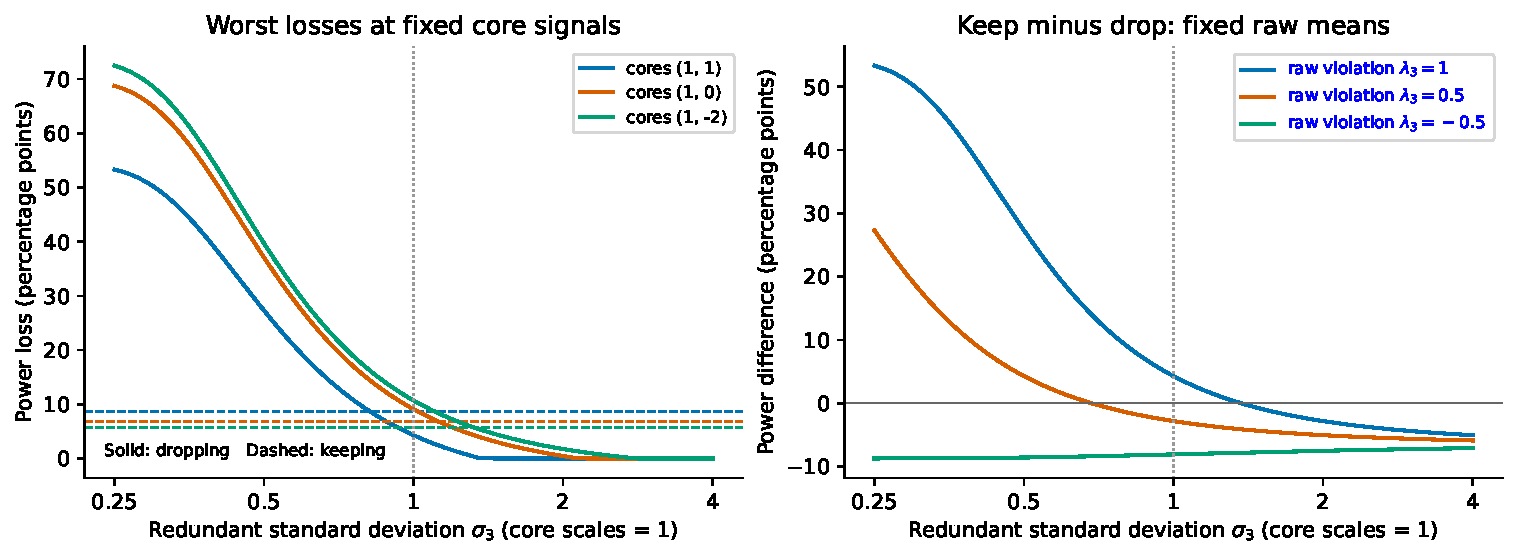
\includegraphics[width=\textwidth]{figures/sec4-pilot-precision.pdf}
\caption{Precision of the redundant moment. Two core inequalities with $\sigma_1=\sigma_2=1$, independent moments, $\alpha=0.10$, and the order imposed on the moments in their original units. Left: largest loss from dropping the redundant inequality (solid) and from keeping it (dashed) as functions of $\sigma_3$, for three pairs of core signals $(\delta_1,\delta_2)$. Right: power of the test that keeps the redundant inequality minus power of the test that drops it, at local violations $\lambda=(1,1,\lambda_3)'$ in the original units, so that $\delta_3=\lambda_3/\sigma_3$.}
\label{fig:precision}
\end{figure}

For the right panel, write $\lambda:=D\delta$ for the local violations in the original units and fix $\lambda_1=\lambda_2=1$ and $\lambda_3\in\{1,\,1/2,\,-1/2\}$. These satisfy the ordering for every $\sigma_3$, and the panel plots $\Delta(\delta)$ at $\delta_3=\lambda_3/\sigma_3$. When $\lambda_3>0$, greater precision increases the redundant signal and the gain from keeping it. Keeping is the better choice when $\sigma_3$ is below approximately $1.37$ if $\lambda_3=1$, and below approximately $0.68$ if $\lambda_3=1/2$. When $\lambda_3<0$, greater precision makes the inequality more clearly slack. With $\lambda_3=-1/2$, keeping costs between $7$ and $9$ points over the range shown.

The third inequality remains redundant for identification. Greater precision can nevertheless make dropping it substantially more costly. The largest cost of keeping is unchanged, although the loss at a particular alternative need not be.

\clearpage
%%%%%%%%%%%%%%%%%%%%%%%%%%%%%%%%%%%%%%
\bibliography{redundant.bib}
%%%%%%%%%%%%%%%%%%%%%%%%%%%%%%%%%%%%%%

\end{document}
